%Når du starter på en opgave skriver du \begin{opgave}{navnet på opgaven}{sværhedsgrad}, hvor sværhedsgraden skrives som 1,2 eller 3, hvor 3 er den sværeste. 
%Når opgaven er slut skrives \end{opgave}. 
%Såfremt der er delopgaver skrives delopgaver som \opg 

%Eksempel på opgave 
%\begin{opgave}{Polære koordinater}{1}
  %Den kinetiske energi af et legeme, der bevæger sig i 2D-planet er
  %i kartesiske koordinater ($x$ og $y$) givet ved ligning
  %(1.11).
  %
  %\opg Beregn $\dt{x}$ og $\dt{y}$ i polære koordinater og vis
  %derefter, at den kinetiske energi udtrykt i polære koordinater er
  %givet ved ligning (1.12).
%\end{opgave}

\chapter{Kerne-- og Partikelfysik Opgaver}

\section*{Kernefysik}
\begin{opgave}{Alfa-henfald}{1}
Alfa-henfald, hvor der udsendes en heliumkerne er en almindelig type henfald. F.eks. følgende henfald af Uran-238
\begin{equation*}
^{238}_{92} \text{U} \rightarrow ^{232}_{90}\text{Th} + ^{4}_{2}\text{He} .
\end{equation*}
\opg Hvorfor tror du netop udsendelsen af en alfa-partikel er en favoriseret type henfald? 
\opg Hvad er reaktionens $Q$-værdi? Ville denne reaktion forekomme naturligt?
Du kan anvende følgende atomare masser:
\begin{align*}
M(^{238}\text{U}) &=238,05079~\SI{}{u} \\
M(^{234}\text{Th}) &= 234,04360~\SI{}{u} \\
M(^4\text{He}) &= 4,002602~\SI{}{u} \\
\end{align*}
.
\end{opgave}

\begin{opgave}{Berylliums isotoper}{2}
Det lette grundstof beryllium har i alt otte isotoper, hvoraf kun Be-9 er stabil. \\
\opg Sammenlign den atomare masse af Be-8 med massen af to He-4. Hvad kan man konkludere herfra? 
\opg Sammenlign også den atomare masse af Be-9 med massen af $^7\text{Li}$ og $^2\text{H}$. Hvad fortæller dette dig?

Du kan anvende følgende masser:
\begin{align*}
M(^2\text{H}) &= 2,014102~\SI{}{u}\\
M(^4\text{He}) &= 4,002602~\SI{}{u} \\
M(^7\text{Li}) &= 7,016003~\SI{}{u} \\
M(^8\text{Be}) &= 8,005305~\SI{}{u} \\
M(^9\text{Be}) &= 9,012174~\SI{}{u}
\end{align*} 
\end{opgave}

\begin{opgave}{Kerners tæthed}{3}
\label{opg:density}
En atomkerne kan antages at være en kugle, sådan at volumen er givet som $V=\frac{4}{3} \pi R^3$. Vis, at tætheden af en kerne ikke afhænger af grundstoffet, altså at tætheden er ens for alle kerner. \emph{Hint: anvend at massen af en kerne i atomare masseenheder ca. er lig massetallet for kernen, altså at $m\approx A$}.
\end{opgave}

\begin{opgave}{Den stærkest bundne kerne}{1}
\label{opg:nickel}
$^{62}\text{Ni}$ har den højeste bindingsenergi per nukleon af alle kerner. 
\opg Hvor meget energi skal der til for at splitte kernen ad?
Anvend at den atomare masse af $^{62}\text{Ni}$ er $61,928349~\SI{}{u}$.
\end{opgave}

\begin{opgave}{Splittelsen af en kerne}{1}
Antag følgende reaktion:
\begin{equation*}
^{28}_{14} \text{Si} + \gamma \rightarrow ^{24}_{12}\text{Mg} + X,
\end{equation*}

hvor $X$ er en kerne.
\opg hvad er $A$ og $Z$ for $X$?
\opg hvis vi antager at energien af fotonen ikke går til kinetisk energi for $^{24}_{12}\text{Mg}$ og $X$, hvad er så dens energi? Anvend at massen af et Si-28-atom er $27,976927~\si{u}$ og at massen af et Mg-24-atom er $23,985042~\si{u}$
\end{opgave}

\begin{opgave}{Fusion i Solen}{2}
Stjerner som Solen skinner på grund af den fusion som foregår i deres kerner. Temperaturen i stjernernes kerner er så høje, at elektronerne er frie, altså ikke bundet til atomer. I Solen omdannes 4 protoner gennem en række skridt (kaldet pp-kæden) til én $^{4}\text{He}$-kerne. Helt overordnet kan reaktionen skrives som:
\begin{equation*}
4p \rightarrow \alpha + 2e^+ + 2\nu_e + E,
\end{equation*}
Dvs. der bliver desuden dannet to positroner og 2 elektronneutrinoer samt en mængde energi.
\opg Hvor meget energi dannes i ovenstående reaktion? Antag at elektronneutrinoens masse er 0. Du kan anvende \emph{ den atomare masse} af helium: $M(^4\text{He})= 4,002602~\SI{}{u}$.
\opg pp-kæden starter ved at to protoner mødes. Men i kraft af deres ladning vil de frastøde hinanden, og de skal derfor have tilstrækkelig bevægelsesenergi for at det kan lade sig gøre. Det elektriske potential (barrieren) mellem to ladede partikler er givet ved:
\begin{equation}
U = \frac{1}{4\pi \epsilon_0} \frac{q_1q_2}{r}.
\end{equation}
Potentialet $U$ er i joule, hvis ladningerne af partiklerne angives i coulomb.
Antag at den stærke kernekraft overvinder den elektriske frastødning når de to protoner kommer i afstanden af $1,4 \cdot 10^{-15}$m fra hinanden. Hvad er den samlede minimale energi af protonerne?
\opg Det er kun muligt for atomer og partikler at have så høje energier ved virkelig høje temperaturer. Den gennemsnitlige energi af partikler og temperaturen af det medie, de befinder sig i, er relateret til hinanden via:
\begin{equation}
E = \frac{3}{2} k T,
\end{equation}
hvor $k$ er Boltzmanns konstant og $T$ er temperaturen i grader Kelvin. Hvad er temperaturen svarende til energien du fandt i foregående opgave? Solens kernetemperatur er ca. $1,5 \cdot 10^7$K. Hvordan sammenlignes det med dit resultat?
\opg NB: sjov opgave!
Vi kan prøve at antage, at al energien der bliver produceret i ovenstående reaktion bliver båret væk af neutrinoer. Lad os også antage at al Solens udstråling bliver skabt ved ovenstående reaktion. Ved Jordens overflade modtages Solens udstråling (kaldet solkonstanten $S_0$) ved værdien: $S_0 = 1,362 \cdot 10^3 J m^{-2}s^{-1}$. Hvor mange neutrinoer fra Solen rammer en kvadratcentimeter af Jordens overflade hvert sekund? Hvor mange solneutrinoer rammer spidsen af din finger hvert sekund?
\end{opgave}

\begin{opgave}{Dannelse af tunge grundstoffer i en supernova: r- og s-proces}{2}
Stjerner kan kun fusionere grundstoffer op til jern. Figur \ref{fig:fusion} viser tværsnittet af en tung stjerne som befinder sig i slutningen af dens levetid.
\begin{figure}[h]
  \centering
  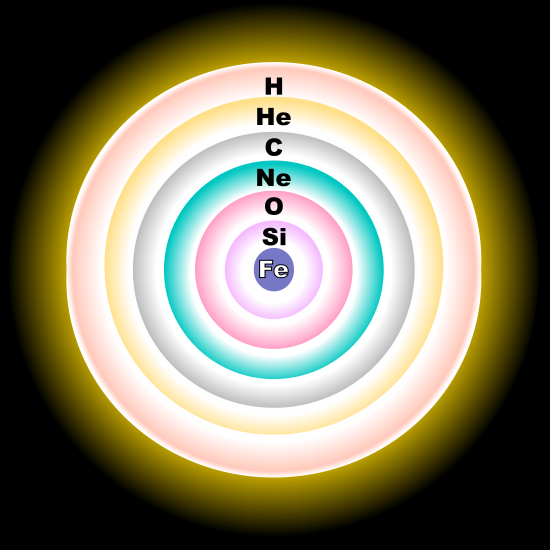
\includegraphics[scale=0.3]{KernePartikel/fusion.png}
  \caption{Skalstruktur i stjerner}
  \label{fig:fusion}
\end{figure}
\opg Forklar løgstruktur-udseendet af stjernen. Hvad er grunden til at stjerner ikke kan danne elementer tungere end jern ved fusion?

Elementer tungere end jern må da være dannet andetsteds end i stjernernes indre. Et miljø, hvor der dannes tunge grundstoffer er de energirige supernova-eksplosioner. Her bliver grundstofferne ikke dannet ved fusion, men ved neutron-indfangning og senere $\beta^-$-henfald af kernen. Det kunne f.eks. foregå på følgende måde:
\begin{equation*}
^{A}_{Z} \text{X}_{N} + n \rightarrow  ^{A+1}_{Z}\text{X}_{N+1} \rightarrow ^{A+1}_{Z+1}\text{Y}_{N} + e^- + \bar{\nu}_e
\end{equation*}

I en supernova-eksplosion skabes en kæmpe mængde neutroner, som gør neutron-indfangning muligt. Men kerner med ekstra neutroner er ustabile og vil henfalde ved hjælp af $\beta^-$-henfald. Derfor kan man sige, at neutron-indfangningen og henfaldene konkurrerer med hinanden. Hvis neutron-indfangningen kan ske hurtigere end kernen kan nå henfalde kaldes det for en r-proces ("r" for \emph{eng: rapid} - hurtig). Hvis kernen når at henfalde inden den kan indfange en ny neutron kaldes det for en s-proces ("s" for \emph{eng: slow} - langsom). \\

Figur \ref{fig:sn} viser et udsnit af kernekortet omkring $N \sim 100$ og $Z \sim 70$. 


De sorte firkanter repræsenterer kerner som er stabile, og derfor ikke kan undergå henfald. 
\opg Hvordan ændrer en kerne sig på kortet hvis den fanger én neutron? Hvordan ændrer en kerne sig på kortet hvis den undergår $\beta^-$-henfald?
\opg Start ved kernen 181-Ta. Antag at kernen undergår 5 neutron-indfangninger ved r-proces. Hvilken kerne bliver dannet (til sidst?)
\opg Antag nu at kernen undergår 5 neutron-indfangninger ved s-proces. Hvilken kerne bliver dannet?
\opg Kan kernen 180-Ta dannes ved neutronindfangning? Forklar dit svar.
\end{opgave}
\begin{figure}[h]
	\centering
	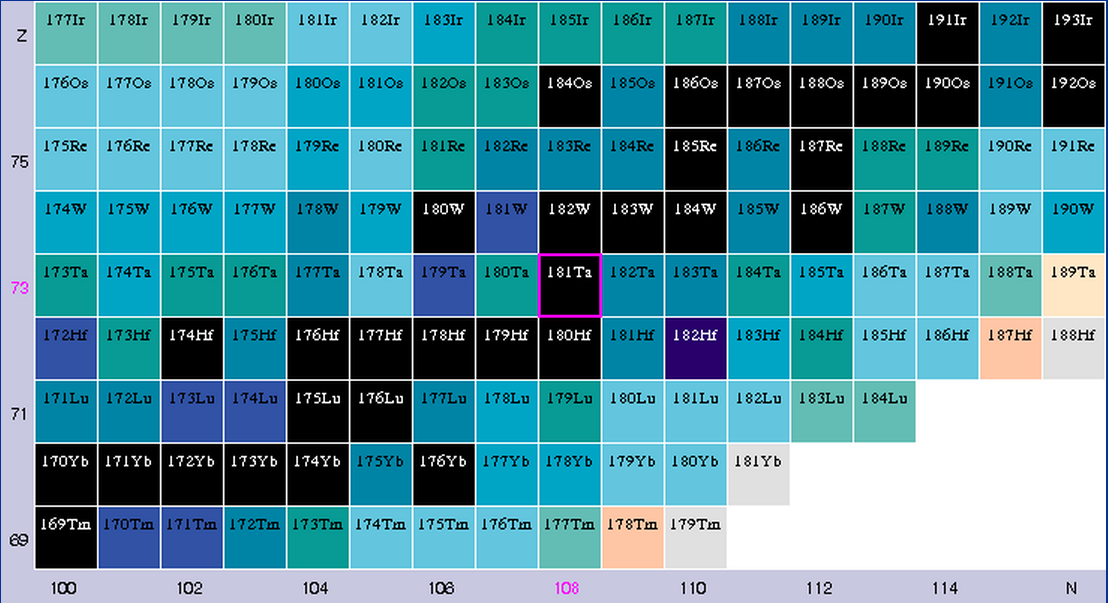
\includegraphics[width=\textwidth]{KernePartikel/supernova_chart.png}
	\caption{Et udsnit af kernekortet}
	\label{fig:sn}
\end{figure}
\newpage

\section*{Partikelfysik}

\begin{opgave}{Bevarelseslove}{1}
\opg Hvilke bevarelseslove gør sig gældende i partikelfysik?\\
\opg Kig på følgende reaktioner og bestem, om de kan lade sig gøre eller ej.
\begin{enumerate}
\item $e^- \longleftrightarrow e^- + e^+ + e^+$
\item $p + n \longleftrightarrow e^- + e^+ + e^+$
\item $p + n + e^+ \longleftrightarrow n + p + \bar{\nu}_e$
\item $p \longleftrightarrow \mu^- + n + \bar{\nu}_\mu $
\item $p \longleftrightarrow \mu^+ + n + \nu_\mu $
\item $\bar{n} \longleftrightarrow \bar{p} + e^+ + \nu_e$
\item $e^- + \mu^+ \longleftrightarrow n$
\end{enumerate}
\emph{Hint: tjek om bevarelseslovene er opfyldt.}
\end{opgave}

\begin{opgave}{Dannelse af to muoner}{1}
Tegn et feynman-diagram, hvor en foton danner muoner i en pardannelsesproces. Hvad er den minimalt krævede energi af fotonen? 
\end{opgave}

\begin{opgave}{Reaktioner med $W^\pm$-partiklen}{2}
\label{opg:W}
Betragt reaktionen i Figur \ref{fig:Wvertex}.
\begin{figure}[h]
  \centering
  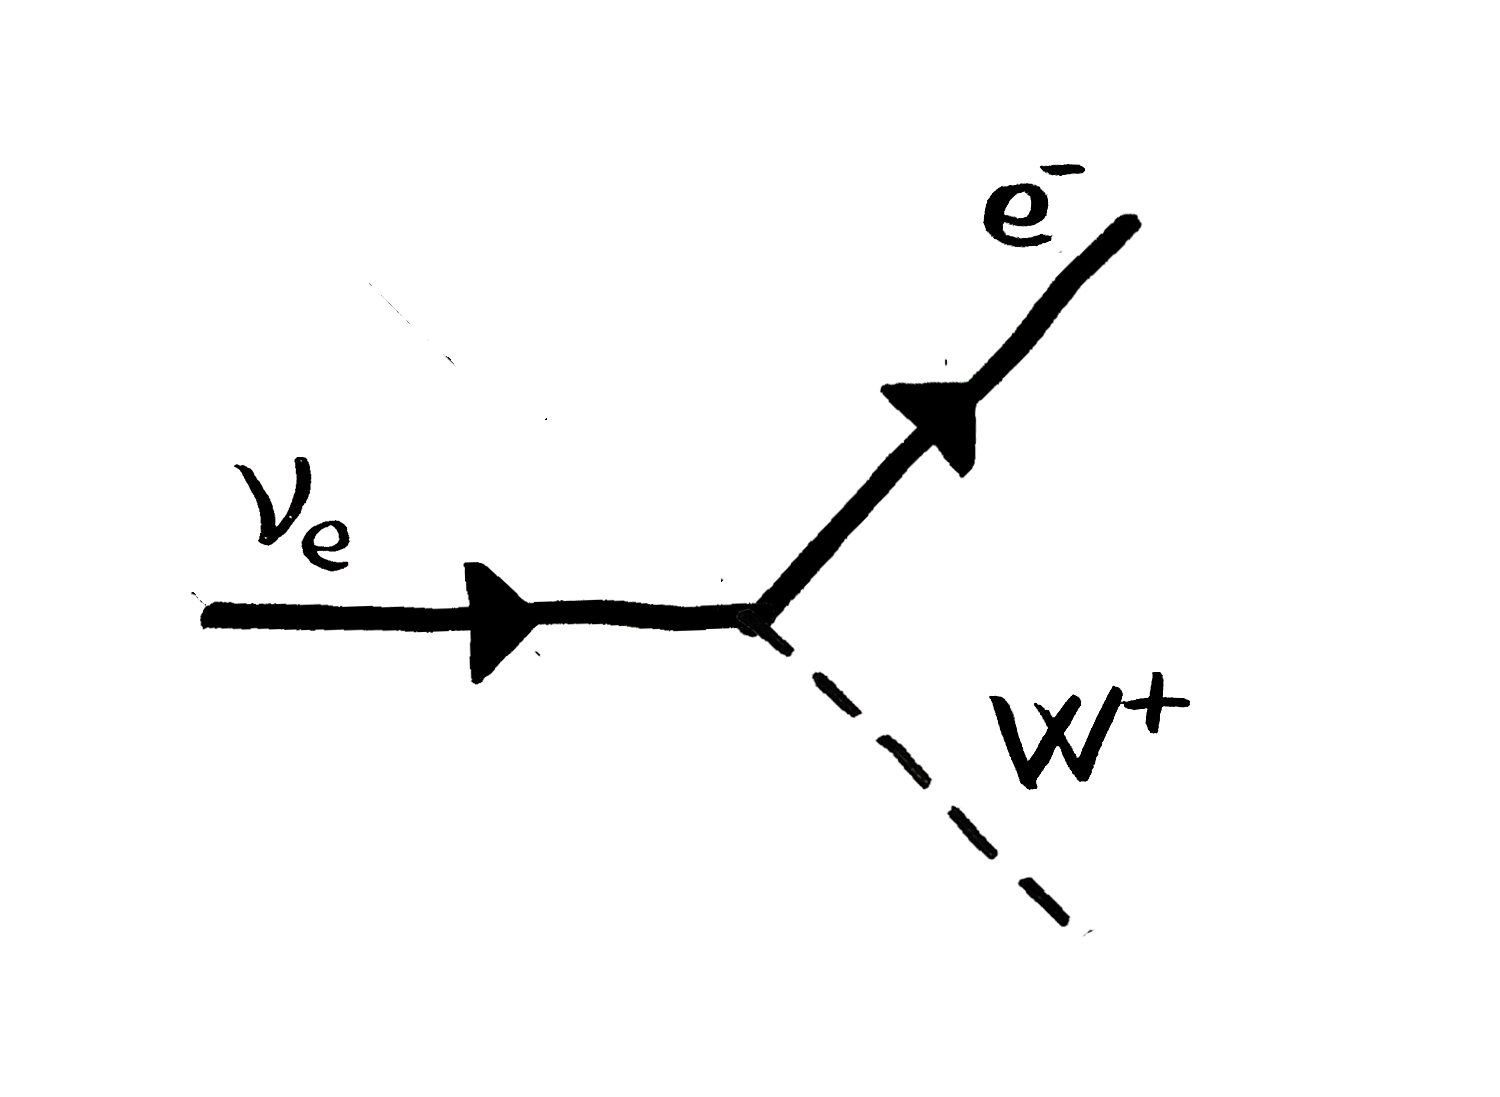
\includegraphics[width=0.3\textwidth]{KernePartikel/weak_vertex.png}
  \caption{Udsendelse af en $W^+$-boson.}
  \label{fig:Wvertex}
\end{figure}
\opg
Rotér feynmandiagrammet mod uret så det viser en indkommende positron i stedet. Hvad slags neutrino produceres der? Hvad er nu ladningen af $W$-bosonen?
\opg
Udskift positronen med en elektron. Hvad slags neutrino produceres der og hvad er ladningen af $W$-bosonen?

Feynman--diagrammet for et beta--minus--henfald er vist
i Figur \ref{fig:beta_minus}.
\begin{figure}[h]
  \centering
  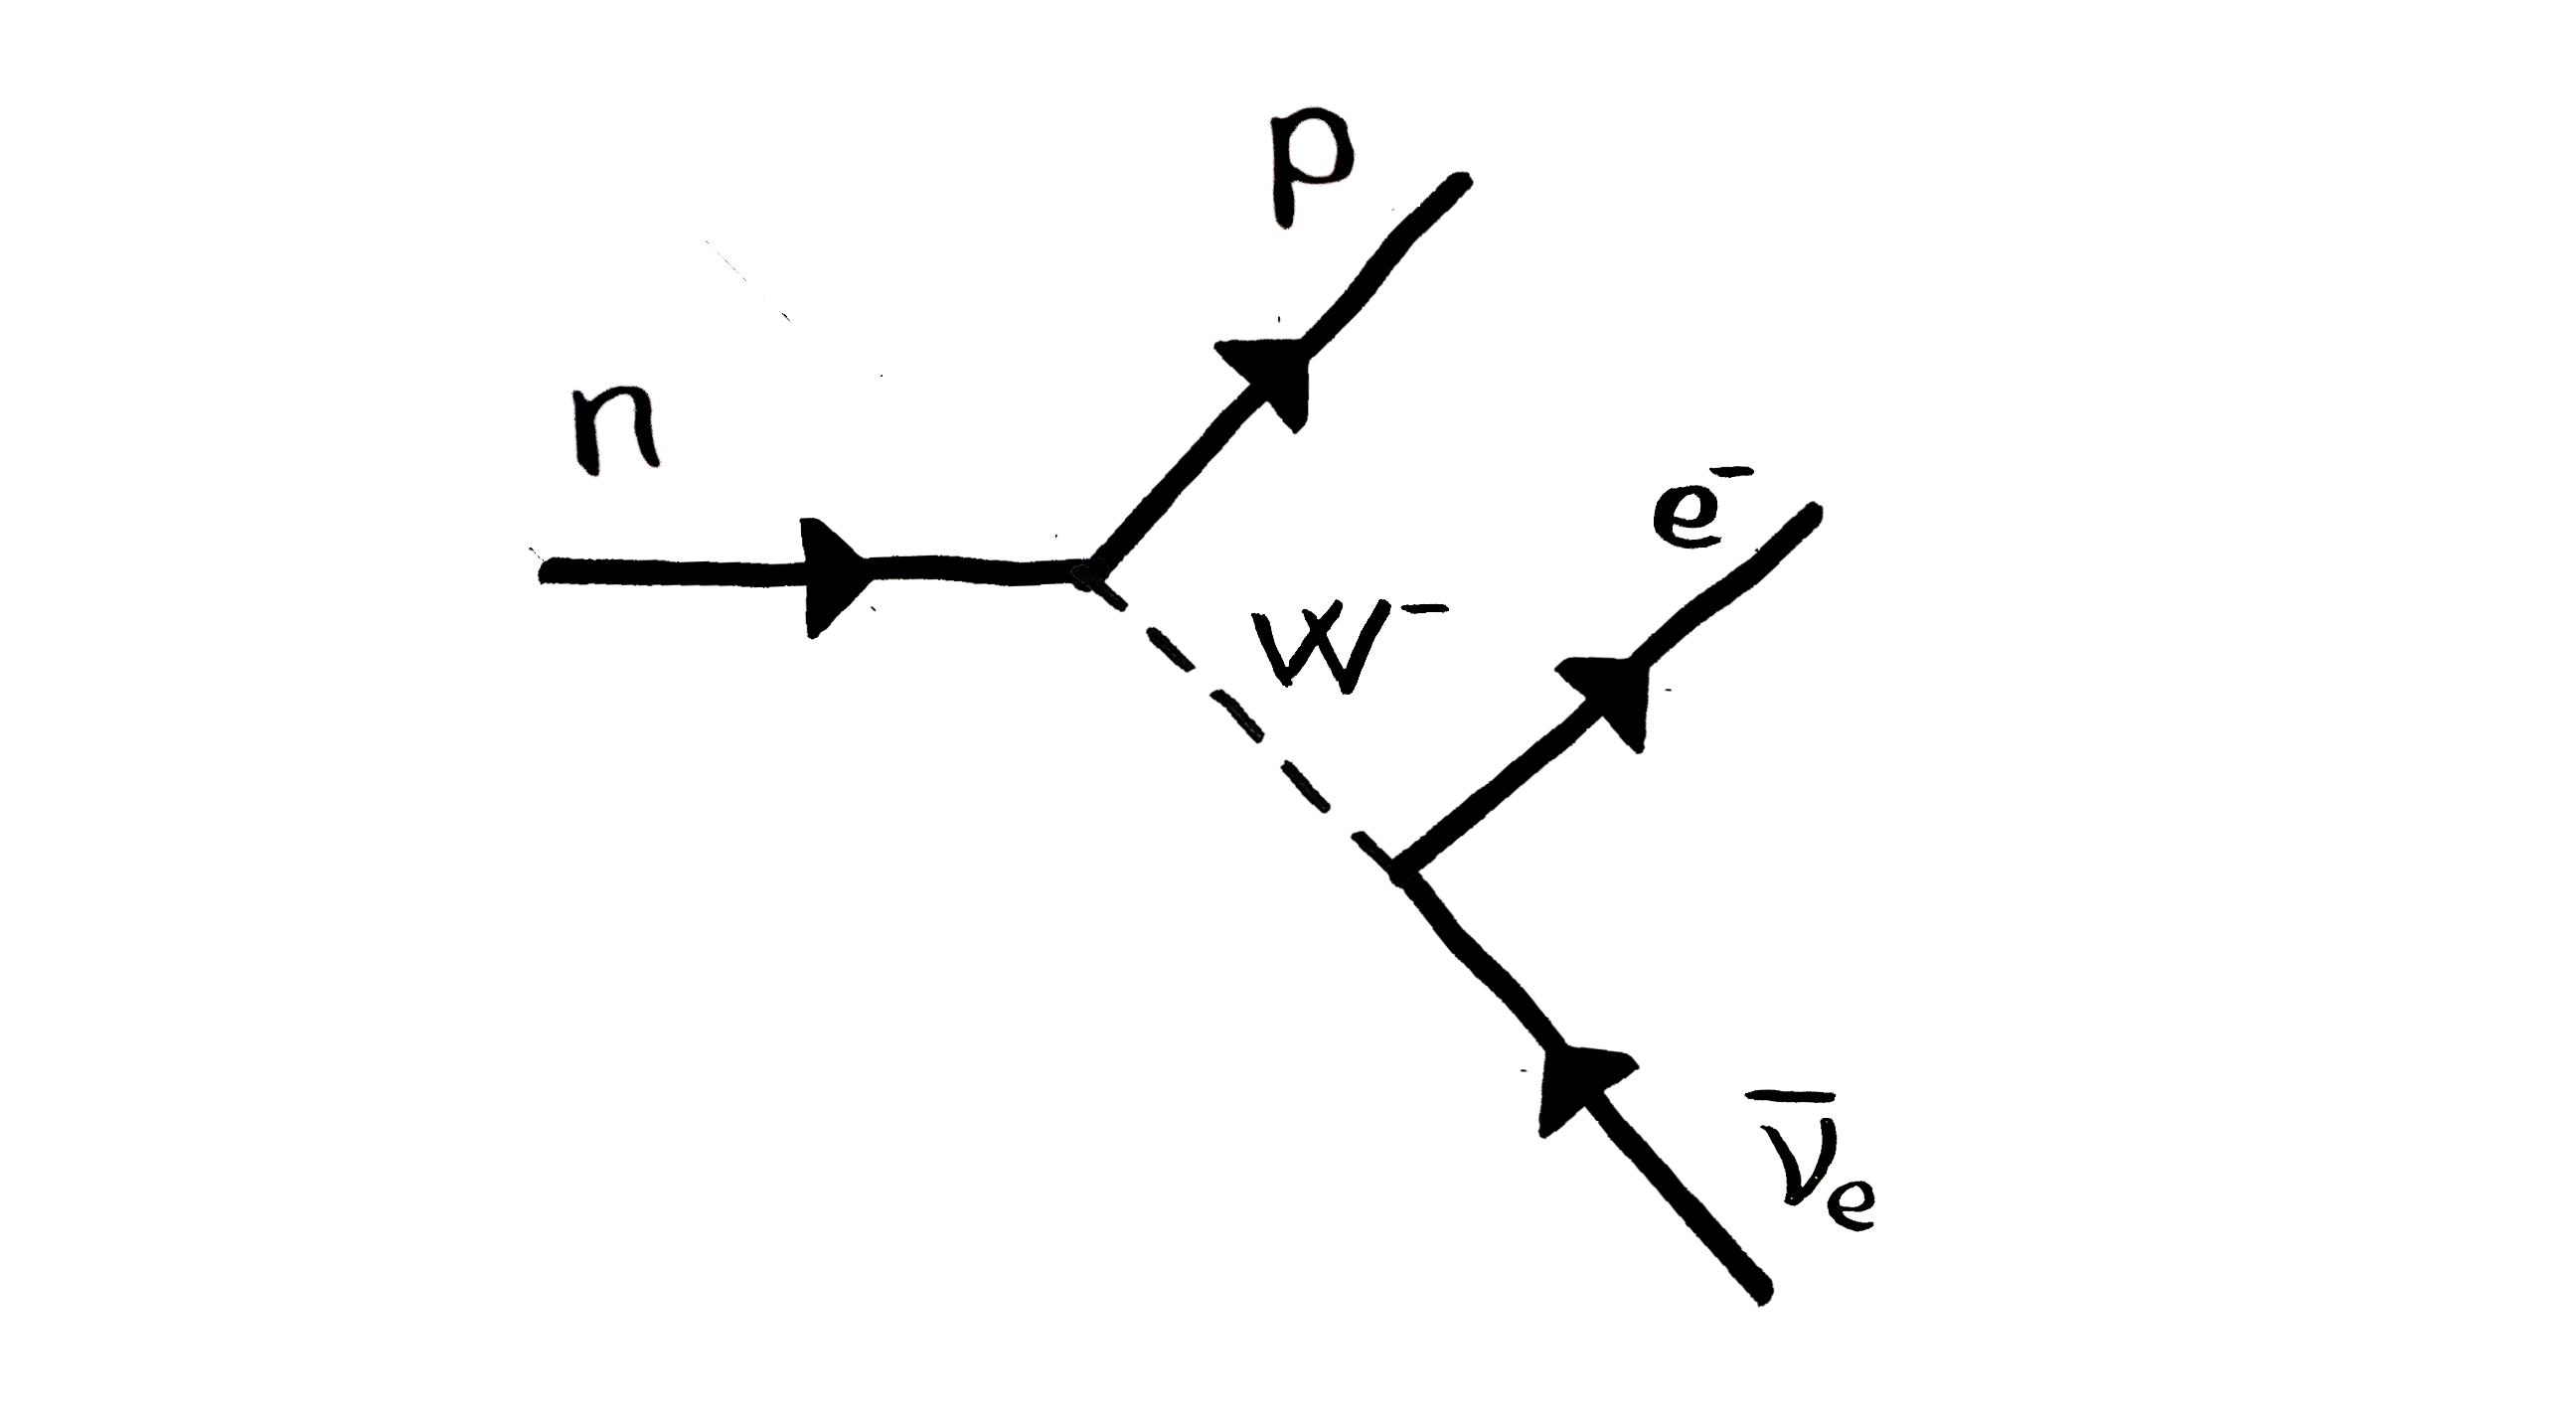
\includegraphics[width=0.6\textwidth]{KernePartikel/beta_minus.png}
  \caption{Beta-minus-henfald.}
  \label{fig:beta_minus}
\end{figure}
\opg Tegn feynman-diagrammet for et beta-plus-henfald: $p \rightarrow
n + e^+ + \nu_e$.
\opg Tegn feynman-diagrammet for en elektron-indfangning: $p + e^-
\rightarrow n + \nu_e$.

Som nævnt i kompendiet består neutronen og protonen af kvarker, som kan omdannes ved hjælp af $W$-bosonen, så deres ladningen ændres med enten $\pm$ 1, f.eks. u$\longleftrightarrow$ d. Figur \ref{fig:Wquarks} viser en oversigt over kvarkerne, hvor pilen mellem u-- og d-- kvarken betyder, at $W$-bosonen kan ændre disse kvarker til hinanden. 
\begin{figure}[h!]
  \centering
  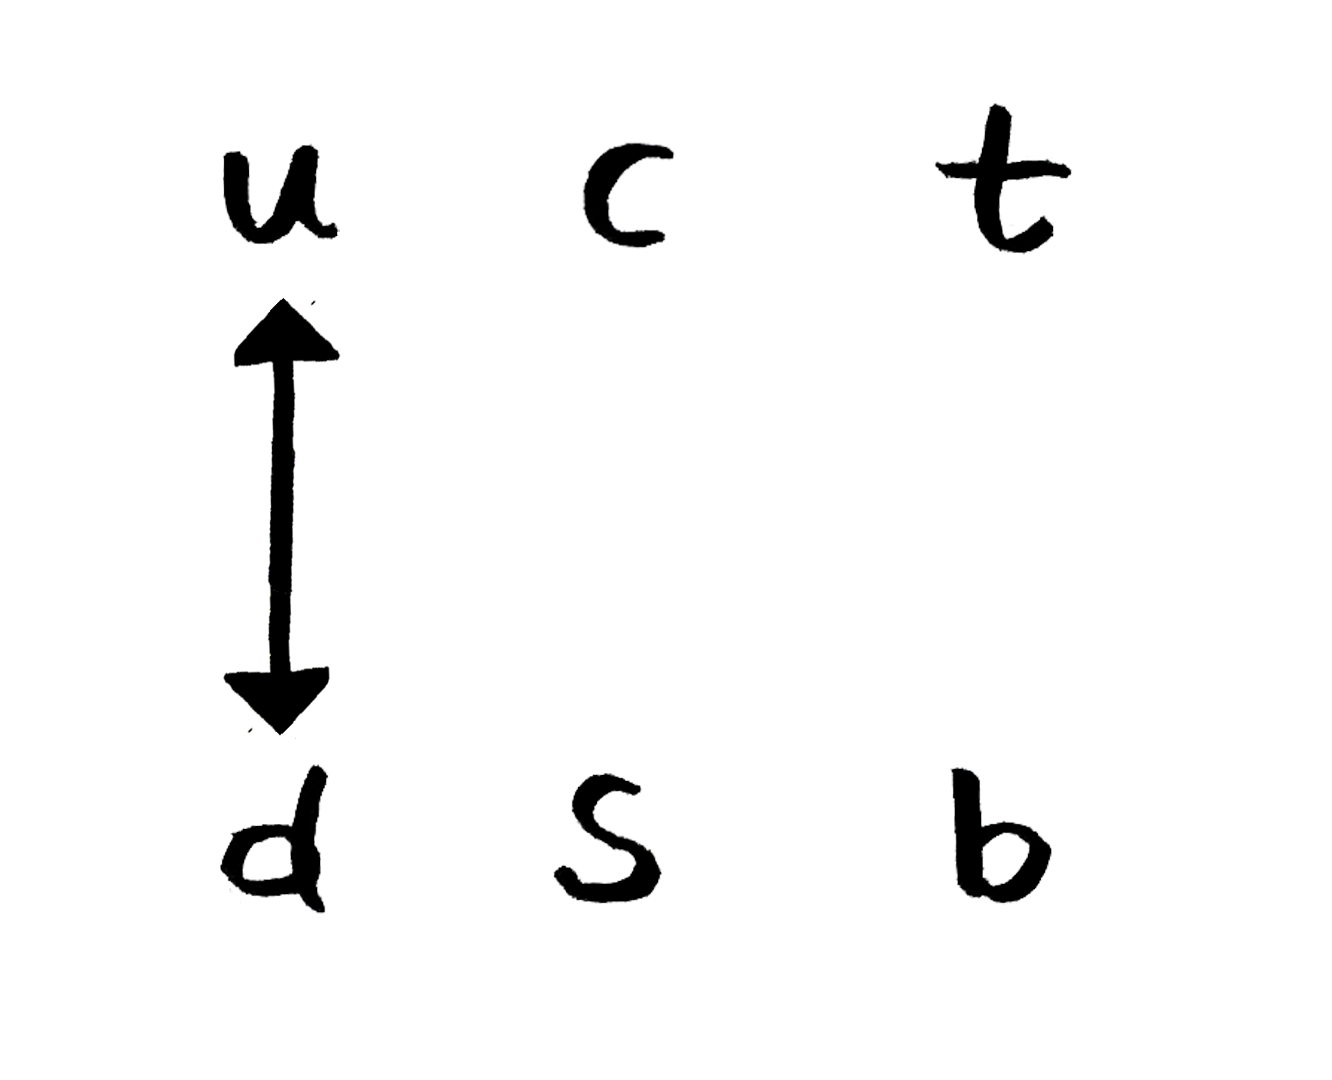
\includegraphics[width=0.3\textwidth]{KernePartikel/Wquarks.png}
  \caption{$W$-bosonen kan ændre kvarker til en anden type så længe ladningen ændres med $\pm 1$}
  \label{fig:Wquarks}
\end{figure}
\opg Indtegn på figur \ref{fig:Wquarks} pile mellem alle de kvarker, som $W$ kan omdanne. 
\opg En t-kvark omdannes til en b-kvark under udsendelse af en $W$-partikel. Tegn feynman-diagrammet. Hvad er ladningen af $W$?
\opg En s-kvark og en anti-c kvark annihilerer og skaber en $W$-partikel. Tegn feynman-diagrammet. Hvad er ladningen af $W$?
\opg Tegn feynmandiagrammet for et beta-minus-henfald, men denne gang tegn neutronens og protonens kvarker som en del af reaktionen. \emph{Hint: partikler kan sagtens optræde uændret i et feynman-diagram.}
\end{opgave}

\begin{opgave}{Feynman-diagrammer: en sand kunstart}{3}
\label{opg:feynman1}
\emph{NB: det er en god idé at lave opgave \ref{opg:W} inden denne opgave.}

Før vi er helt klar til at give os i kast med en masse
feynman-diagrammer, skal gluonen ($g$) introduceres. Gluonen, som
bærer den stærke vekselvirkning, virker ved at ændre en egenskab ved
kvarkerne kaldet \emph{farve}. Feltet som beskæftiger sig med dette
kaldes for kvantekromodynamik, og det er det, som beskriver hvorfor
kvarkerne kun kan eksistere i grupper af tre (hadronerne) og to
(mesonerne). Kvantekromodynamik er dog en anelse ud over niveauet for
denne camp, men det forhindrer os ikke i at gøre brug af gluonen i
vores feynman-diagrammer.
\begin{figure}[h!]
  \centering
  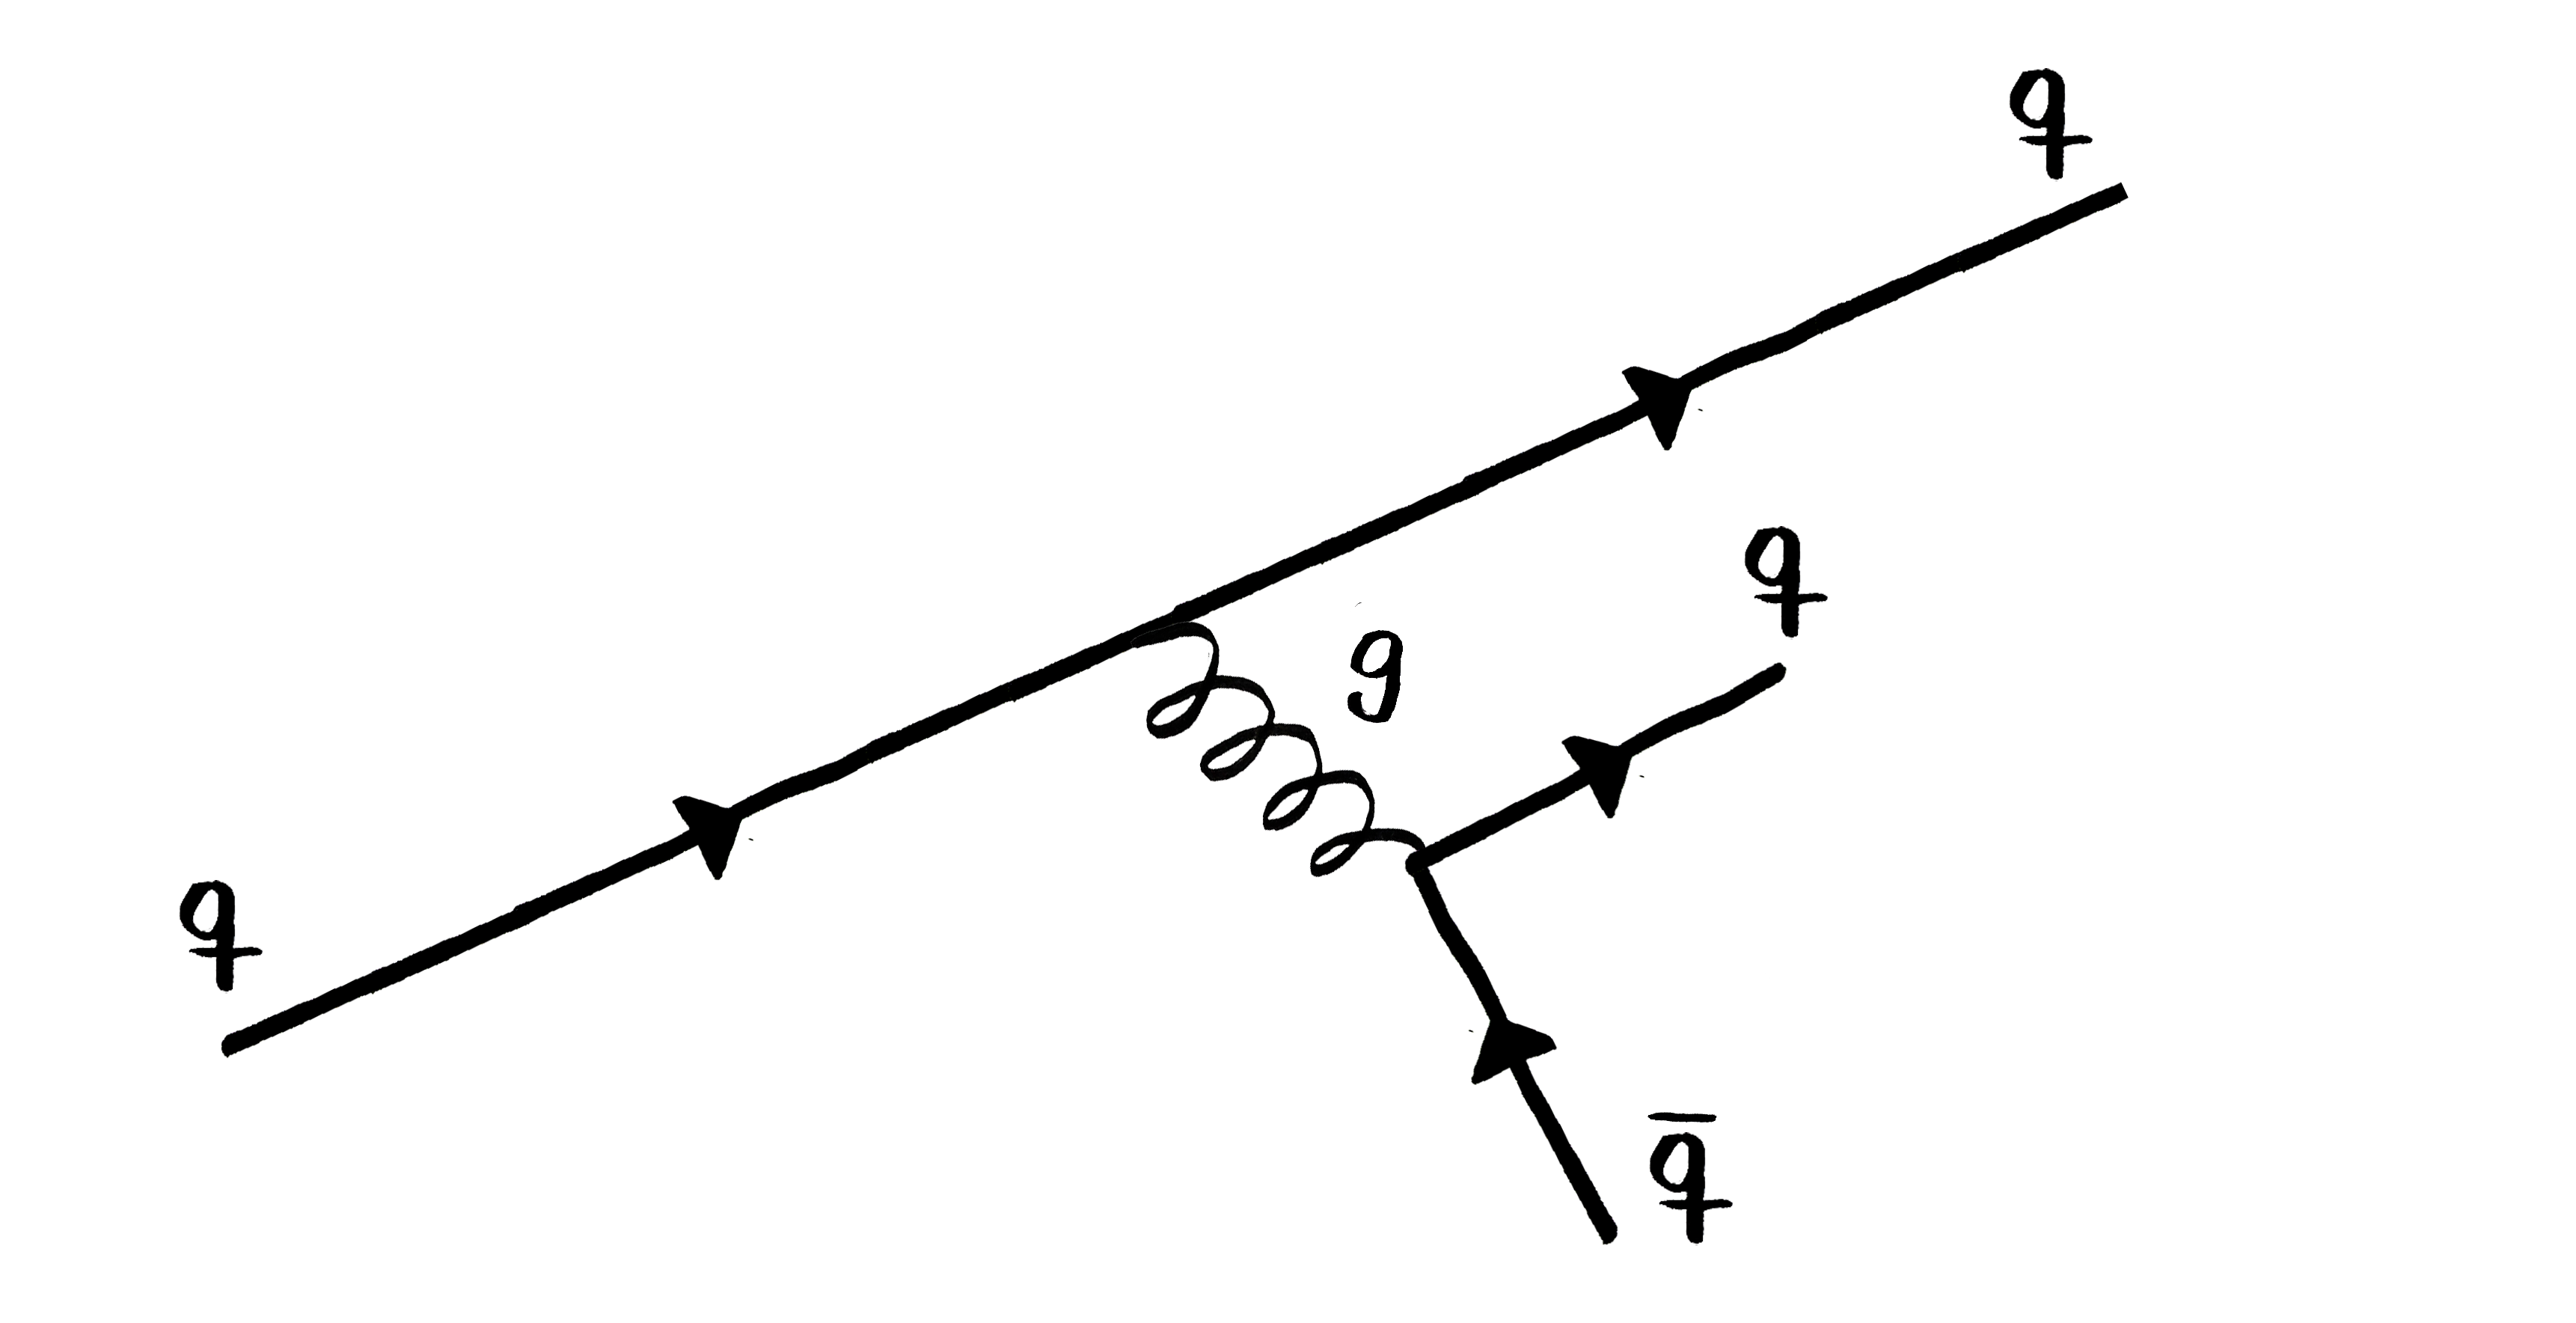
\includegraphics[width=0.6\textwidth]{KernePartikel/quark_interaction.png}
  \caption{Reaktion med gluonen $g$.}
  \label{fig:quark_inter}
\end{figure}
Figur \ref{fig:quark_inter} viser en typisk vekselvirkning med
gluonen, som normalt tegnes som en fjederform. Heri udsender en
vilkårlig kvark en gluon og fortsætter. Kvarktypen ændrer sig ikke
under udsendelse af en gluon (kun dens farve, men igen, det behøver vi
ikke tage højde for). Gluonen henfalder til et vilkårligt
kvark-antikvark-par. Gluonens energi afgør, hvilket
kvark-antikvark-par der kan dannes, men u- og d-kvarken er de mindst
energirige (mindst massive) og kan derfor altid dannes med høj
sandsynlighed. Det betyder, at det er ''gratis'' at introducere en gluon
i dit feynman-diagram, som enten henfalder til et u$\bar{\text{u}}$-
eller d$\bar{\text{d}}$-par.

Nu skal vi sætte vores nylærte
egenskaber til prøve med henfald af sammensatte partikler. Som
eksempel kigger vi på henfaldet:
\begin{equation*}
D^- \rightarrow K^+ + \pi^- + \pi^-.
\end{equation*}
Dette er henfaldet af $D^-$-mesonen (kvarksammensætning: d$\bar{\text{c}}$ ) til mesonerne $K^+$ (u$\bar{\text{s}}$), og to $\pi^-$ (d$\bar{\text{u}}$). Et sådant henfald er vist i figur \ref{fig:D_reaction}. Læg mærke til, at man kan sætte klammer om de kvarker, der hører sammen i en partikel.
\begin{figure}[h!]
  \centering
  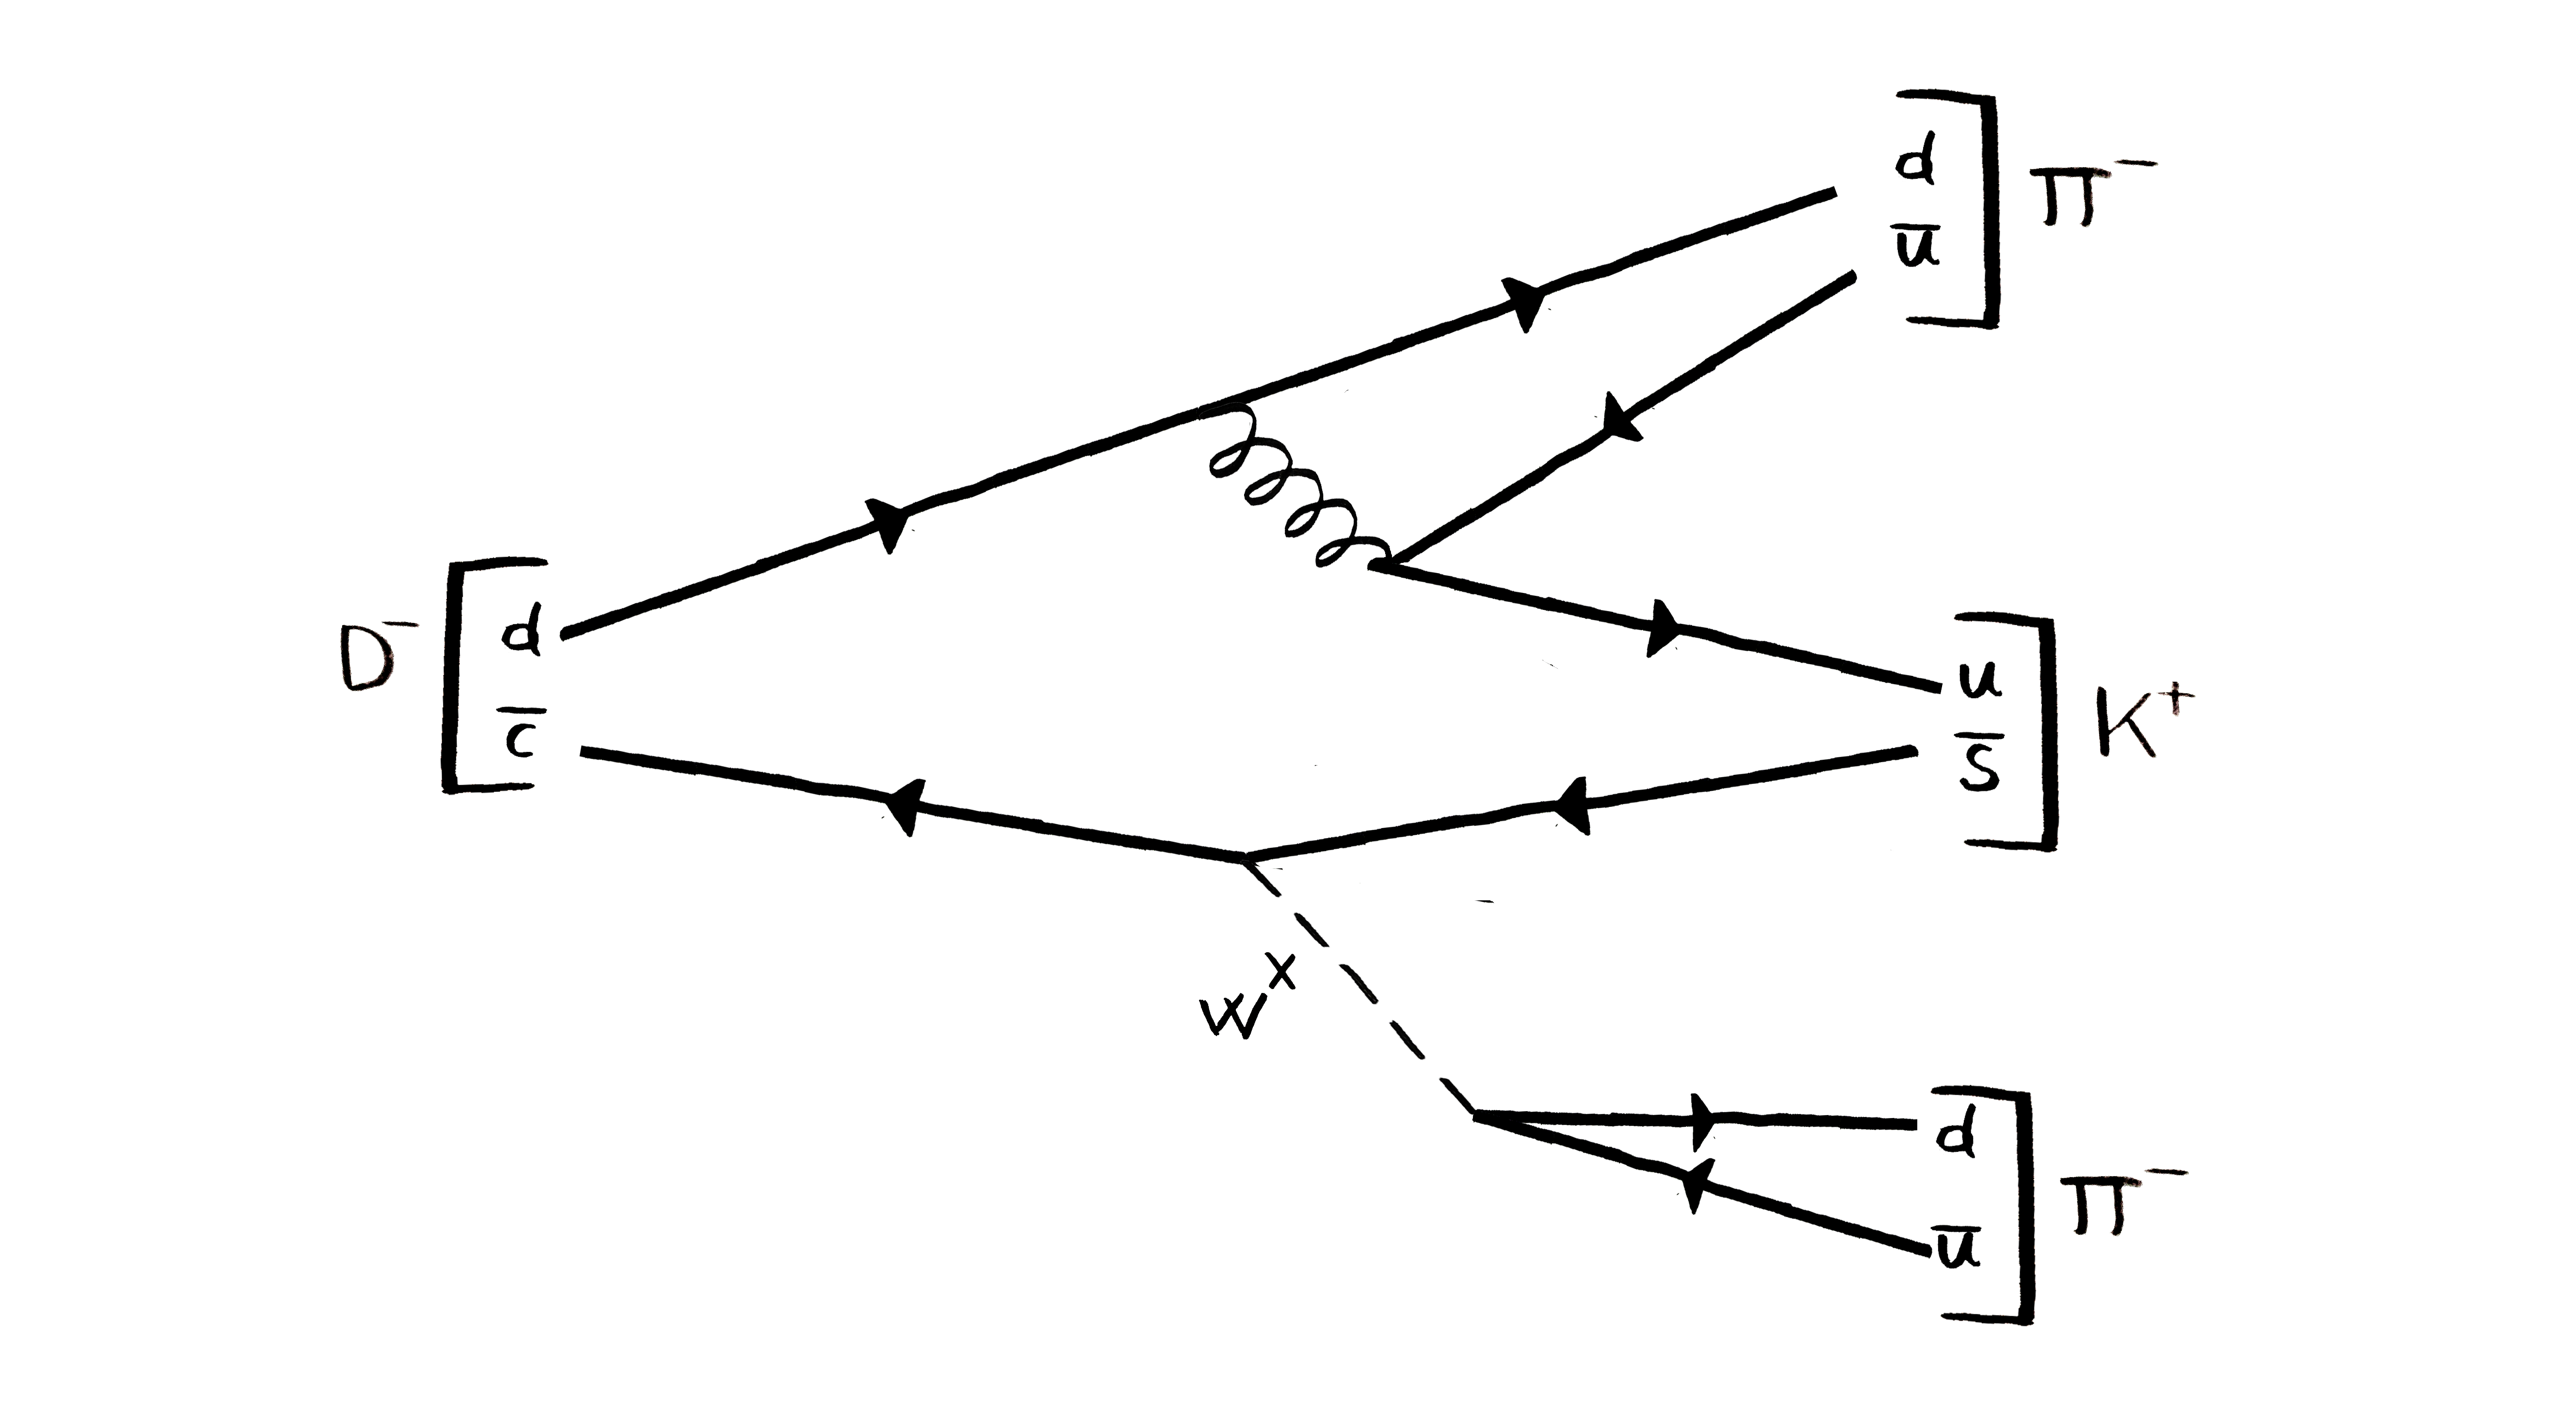
\includegraphics[width=0.8\textwidth]{KernePartikel/reaction3.png}
  \caption{Henfaldet af $D^-$.}
  \label{fig:D_reaction}
\end{figure}
Udfordringen består i at lave et feynman-diagram som er så overskueligt som muligt (f.eks. uden krydsende pile) og som gør brug af \emph{mindst mulige vertexer og derved virtuelle partikler}. Fysisk set betyder færre vertexer = større sandsynlighed.
\opg Hvad er ladningen af $W$-bosonen i figur \ref{fig:D_reaction}?
\opg Beskriv med ord hvad der sker med hver af kvarkerne i $D^-$-mesonen.
\opg Prøv at lave et feynman-diagram for henfaldet: $D^- \rightarrow K^- + \pi^+ + \pi^-$. \emph{Hint: start med at finde kvarksammensætningen af partiklerne.}
\end{opgave}

\begin{opgave}{Relativistiske partikler}{2}
Partikelacceleratorer gør brug af, at partikler kan opnå kæmpe energi ved at blive accelereret op i nærheden af lysets hastighed $c$. Hvis en observatør målte massen af en partikel med hastigheden $v$, ville han måle en større masse end den masse partiklen har, hvis den er i hvile. Man kan vise, at den masse som observatøren måler (kaldet den relativistiske masse, $m_\text{rel}$) er relateret til partiklens hvilemasse $m$ og hastighed $v$ gennem:
\begin{equation}
m_\text{rel} = \frac{m}{\sqrt{1-v^2/c^2}}
\end{equation}
\opg I en bestemt accelerator accelereres elektroner ($m=0,511\SI{}{Mev/c^2}$) op sådan at deres energi bliver $E=580$Mev. Brug $E=m_\text{rel}c^2$ til at finde elektronernes hastighed i enheder af lysets hastighed $c$.
\opg Hvad er elektronernes relativistiske masse?
\end{opgave}

\begin{opgave}{Flere feynman-diagrammer}{2}
\emph{NB: det er en god idé at du har lavet opgave \ref{opg:feynman1} inden denne opgave.}

Tegn feynman-diagrammer for følgende henfald. Husk at gøre brug af mindst mulige vertexer.
\opg $B^- (b\bar{u}) \longrightarrow D^0(c\bar{u}) + \rho^-(d\bar{u})$
\opg $\Sigma^-(dds) \longrightarrow \Lambda^0 (uds) + e^- + \bar{\nu}_e$
\opg $\Delta^0 (udd) \longrightarrow p + \pi^- (d\bar{u})$
\opg $D_s^+ (c\bar{s}) \longrightarrow \phi (s\bar{s}) + \rho^+ (u\bar{d})$
\opg $\Omega^-(sss) \longrightarrow \Xi^-(dss) + \pi^0(u\bar{u})$
\end{opgave}

\chapter{Kerne-- og Partikelfysik Facitliste}
\section*{Kernefysik}
\begin{opgave}{Alfa-henfald}{1}
\begin{equation*}
^{238}_{92} \text{U} \rightarrow ^{234}_{90}\text{Th} + ^{4}_{2}\text{He}.
\end{equation*}
\opg Alfa-partiklen har både magiske tal $Z=2$ og $N=2$, og er derfor utroligt stabil. Det er særligt energimæssigt favorabelt at henfalde til en kerne og en alfa-partikel end f.eks. to arbitrære kerner.
\opg Reaktionens $Q$-værdi udregnes som $Q=(M_i - M_f)c^2$. Her er $M_i=M(^{238}_{92} \text{U})$ og $M_f=M(^{232}_{90}\text{Th}+M(^{4}_{2}\text{He}))$. Med masserne opgivet i atomare masse-enheder anvendes det, at der omregnes til energi gennem $1 u = 931,49406\SI{}{MeV/c^2}$. Dette giver:
\begin{equation*}
Q = 4,273695~\SI{}{MeV}
\end{equation*}
$Q$-værdien er positiv, så reaktionen kan forekomme naturligt.
\end{opgave}

\begin{opgave}{Berylliums isotoper}{2}
\opg Den atomare masse af Be-8 sammenlignes med massen af to He-4.  Be-8 er tungere end to He-4 med:
\begin{align*}
\Delta m &= 8,005305~\SI{}{u} - 2\cdot 4,002602~\SI{}{u}  \\
&=1,01 \cdot 10^{-4}\SI{}{u}
\end{align*}
og det er derfor energimæssigt favorabelt for Be-8 at opsplitte i to He-4.\\
\textbf{Evaluering:} Det er også det der observeres eksperimentelt. Processen udløser $0,0941~\SI{}{MeV/c^2}$ i energi.
\opg Forskellen mellem massen af Be-9 og masserne af $^7\text{Li}$ og $^2\text{H}$ er:
\begin{align*}
\Delta m &= 9,012174~\SI{}{u} - (7,016003~\SI{}{u} + 2,014102~\SI{}{u}) \\
&=-1,80 \cdot 10^{-2}~\SI{}{u}.
\end{align*}
Altså er massen af Li-7 og H-2 større end massen af Be-9.\\
Det betyder at opsplittelsen af en Be-9-kerne til en Li-7- og H-2-kerne ikke kan forekomme.\\
\textbf{Evaluering:} Isotopen Be-9 er rigtig nok stabil. 
\end{opgave}

\begin{opgave}{Kerners tæthed}{3}
Tætheden er massen delt med volumen, $\rho=\frac{m}{V}$. Volumen for en kerne, hvis den antages at være kugleformet, er $V=\frac{4}{3} \pi R^3$. Radius af en kerne er $R=R_0 A^{1/3}$. Anvendes $m\approx A$, ses det, at tætheden af en atomkerne kan siges at være:
\begin{align*}
\rho &= \frac{m}{V} \\
&\approx \frac{A}{\frac{4}{3} \pi R_0^3 A} \\
&= \frac{3}{4 \pi R_0^3}
\end{align*}
Massetallet $A$ optræder ikke ovennævnte ligning, og tætheden er derfor uafhængig af, hvilken type kerne man har med at gøre, og er derfor ens for alle kerner.
\end{opgave}

\begin{opgave}{Den stærkest bundne kerne}{1}
\label{opg:nickel}
Den energi der skal til for at splitte $^{62}\text{Ni}$ ($A=62, Z=28$ og $N=34$) er bindingsenergien, $E_B$. Den udregnes ved:
\begin{align*}
E_B &= (-\Delta M )c^2 \\
&= - (M(62,28)-28(m_p + m_e) - 34m_n)c^2 \\
&= 0,585~\SI{}{u}c^2 \\
&= 544,92~\SI{}{MeV}
\end{align*}
Det er den energi, det kræver at splitte Ni-62.
\textbf{Evaluering:} med bindingsenergien per nukleon på ca. $8,8$ er Ni-62 den stærkest bundne kerne.
\end{opgave}


\begin{opgave}{Splittelsen af en kerne}{1}
\begin{equation*}
^{28}_{14} \text{Si} + \gamma \rightarrow ^{24}_{12}\text{Mg} + X,
\end{equation*}
\opg Det ses, at $A$ for $X$ må være $28-24=4$ og $Z=14-12=2$. $X$ er derfor $^{4}_{2} \text{He}$.
\opg Hvis vi antager at energien af fotonen ikke går til kinetisk energi for $^{24}_{12}\text{Mg}$ og $X$, så er dens energi præcis tilsvarende masseforskellen mellem kernerne på hver side af reaktionstegnet. Vi kender massen af et He-atom til at være $4,002602~\SI{}{u}$, mens de andre masser er givet. Energien af fotonen må være:
\begin{align*}
E_\gamma &= (M(24,12)+M(4,2)-M(28,14))c^2 \\
&=0,011~\si{u}c^2 \\
&=10,25~\si{MeV}
\end{align*}
.
\end{opgave}


\begin{opgave}{Fusion i Solen}{2}
\begin{equation*}
4p \rightarrow \alpha + 2e^+ + 2\nu_e + E,
\end{equation*}
Dvs. der bliver desuden dannet to positroner og 2 elektronneutrinoer samt en mængde energi.
\opg Som overslag kan bruges, at massen af en alfa-partikel + massen af to positroner er den atomare masse af He-4, $M(4,2)=4,002602~\SI{}{u}$. Den energi der dannes er $Q$-værdien:
\begin{align*}
Q &= E_i - E_f \\
&= (4m_p - 4,002602~\SI{}{u})c^2 \\
&= 24,7 ~\si{MeV}.
\end{align*}
Ovenstående svar er godtaget. Men hvis man har kendskab til annihilation skal man medtage, at de to positroner vil annihilere med elektronerne i plasmaet. Dette giver (minimum) energien svarende til 4 gange elektronens hvilemasse (idet $2e^+ + 2e^- \rightarrow \gamma$). Dette giver ekstra $2~\si{MeV}$.
\opg For at få enhederne til at stemme skal ladningerne af protonerne angives i coloumb, $1e = 1,60217 \cdot 10^{-19}~\si{C}$ Den minimale energi krævet af protonerne er givet ved:
\begin{align*}
U &= \frac{1}{4\pi\epsilon_0} \frac{q_1q_2}{r} \\
&= \frac{1}{4\pi\epsilon_0} \frac{\left( 1,602 176565 \cdot 10^{-19}~\si{C}\right)^2}{1,4 \cdot 10^{-15}~\si{m}} \\
&= 1,648 \cdot 10^{-13}~\si{J}
\end{align*}
Svaret kan angives i både eV eller J, men vi skal bruge størrelsen i J i næste opgave.
\opg Energien fundet i foregående opgave indsættes i formlen:
\begin{equation*}
E = \frac{3}{2} k T.
\end{equation*}
Temperaturen findes ved:
\begin{align*}
T &= \frac{2}{3} \frac{E}{k} \\
&\approx 8 \cdot 10^9 ~\si{K}.
\end{align*}
Det er temperaturen det kræver før protonerne besidder energien fundet i foregående opgave.
Solens kernetemperatur er ca. $1,5 \cdot 10^7$K - altså meget lavere end den temperatur vi har fundet!

\textbf{Evaluering:} Fusionen af to protoner finder alligevel sted i Solens indre, til trods for den "lave" temperatur. Temperaturen af protonerne følger en fordeling, som topper ved temperaturen $1,5 \cdot 10^7$K. Det betyder at størstedelen af protonerne har denne temperatur. Men det er muligt for protonerne at have både højere og lavere temperaturer end dette - derfor kan fusionen foregå. Det sker bare med meget lavere sandsynlighed. Det er bl.a. det der afgør hvorfor stjerner som Solen har lang levetid!
\opg Solkonstanten er energi i joule der rammer hver kvadratmeter af Jordens overflade per sekund. Omregning fra joule til MeV:
\begin{align*}
\si{J} &= \frac{1}{1,60217 \cdot 10^{-19}} \si{eV} \\
&= \frac{1}{1,60217 \cdot 10^{-19}} \si{eV} \cdot 10^{-6}~\si{MeV/eV} 
\end{align*} 
Vi starter med at omregne til kvadratcentimeter og MeV:
\begin{align*}
S_0 &=1,362 \cdot 10^3~\SI{}{J m^{-2} s^{-1}} \\
&=1,362 \cdot 10^7~\SI{}{J cm^{-2} s^{-1}} \\
&= 1,362 \cdot 10^7~\SI{}{J cm^{-2} s^{-1}} \cdot \frac{1}{1,60217 \cdot 10^{-19}} \si{eV/J} \cdot 10^{-6}~\si{MeV/eV} \\
&\approx 8,5 \cdot 10^{19}~\SI{}{MeV cm^{-2} s^{-1}}
\end{align*}
Hvis al energi fra Solen dannes af ovenstående reaktion, forekommer der $S_0/E$ reaktioner per sekund, hvor $E$ er energien udløst i reaktionen regnet i foregående opgave. Der dannes to neutrinoer per reaktion, så fluxen af neutrioner per kvadratcentimeter per sekund på Jordens overflade er:
\begin{align*}
\Phi_\nu &=2 \frac{S_0}{E} \\
&=2 \frac{8,5 \cdot 10^{19}~\SI{}{MeV cm^{-2} s^{-1}}}{24,7~\SI{}{MeV}} \\
&\approx 7 \cdot 10^{18}~\SI{}{cm^{-2} s^{-1}}
\end{align*}
En fingerspids har ca. areal på $1~\SI{}{cm^2}$. Antal neutrinoer som rammer en fingerspids per sekund er da:
\begin{align*}
\text{antal:} &= \Phi/\text{areal} \\
&\approx 7 \cdot 10^{18}~\SI{}{s^{-1}}
\end{align*}
\textbf{Evaluering:} Dette tal er stærkt overvurderet idet vi antog, at \emph{al} Solens energi blev båret væk af neutrinoer.
\end{opgave}

\begin{opgave}{Dannelse af tunge grundstoffer i en supernova: r- og s-proces}{2}
\opg I kernen fusioneres lettere elementer til tungere. Dette skaber løgstruktur i stjernen med lette elementer yderst og tunge elementer inderst. Bindingsenergien for jern er så høj, at stjernen ikke vinder energi ved at omdanne lettere grundstoffer til jern. Derfor stopper fusionen, når stjernen har opnået en jern-kerne.
\opg Hvis en kerne fanger én neutron, ændrer $N$ sig med +1. Det svarer til at tage ét skridt til højre på kernekortet. Hvis kernen undergår beta-minus-henfald, så falder $N$ med 1 og $Z$ stiger med 1. Det svarer til at tage ét skridt skråt tilbage på kernekortet.
\opg Ved fem r-proces neutronindfangninger svarer det til at gå fem skridt mod højre på kernekortet. Her ender man ved kernen 186-Ta. Herefter henfalder kernen ved beta-minus indtil den når en stabil kerne, dvs. man går skråt tilbage på kernekortet til man rammer en sort firkant. Man ender ved 186-W.
\opg Ved fem s-proces skal der tages et skridt skråt tilbage efter hvert skridt til højre, hvis kernen er ustabil. Her ender man ved 186-Os.
\opg Kernen 180-Ta kan ikke dannes ved neutronindfangning, da den befinder sig på den anden side af stabilitetslinjen.
\end{opgave}

\newpage
\section*{Partikelfysik}

\begin{opgave}{Bevarelseslove}{1}
\opg Følgende bevarelseslove gør sig gældende:
\begin{itemize}
\item Lepton-tal
\item Baryon-tal
\item Energi
\item Impuls
\item Ladning
\end{itemize}
For at tjekke om en reaktion kan lade sig gøre, tjekkes der for bevarelse af lepton-tal, baryon-tal og ladningsbevarelse.
\opg
\begin{enumerate}
\item $e^- \longleftrightarrow e^- + e^+ + e^+$ (ikke tilladt, ladning og lepton-tal)
\item $p + n \longleftrightarrow e^- + e^+ + e^+$ (ikke tilladt, baryon-tal og lepton-tal)
\item $p + n + e^+ \longleftrightarrow n + p + \bar{\nu}_e$ (ikke tilladt, ladning)
\item $p \longleftrightarrow \mu^- + n + \bar{\nu}_\mu $ (ikke tilladt, ladning)
\item $p \longleftrightarrow \mu^+ + n + \nu_\mu $ (tilladt)
\item $\bar{n} \longleftrightarrow \bar{p} + e^+ + \nu_e$ (tilladt)
\item $e^- + \mu^+ \longleftrightarrow n$ (ikke tilladt, baryon-tal og lepton-tal)
\end{enumerate}
.
\end{opgave}

\begin{opgave}{Dannelse af to muoner}{1}
Feynman-diagram, hvor en foton danner muoner i en pardannelsesproces:
\begin{figure}[h]
  \centering
  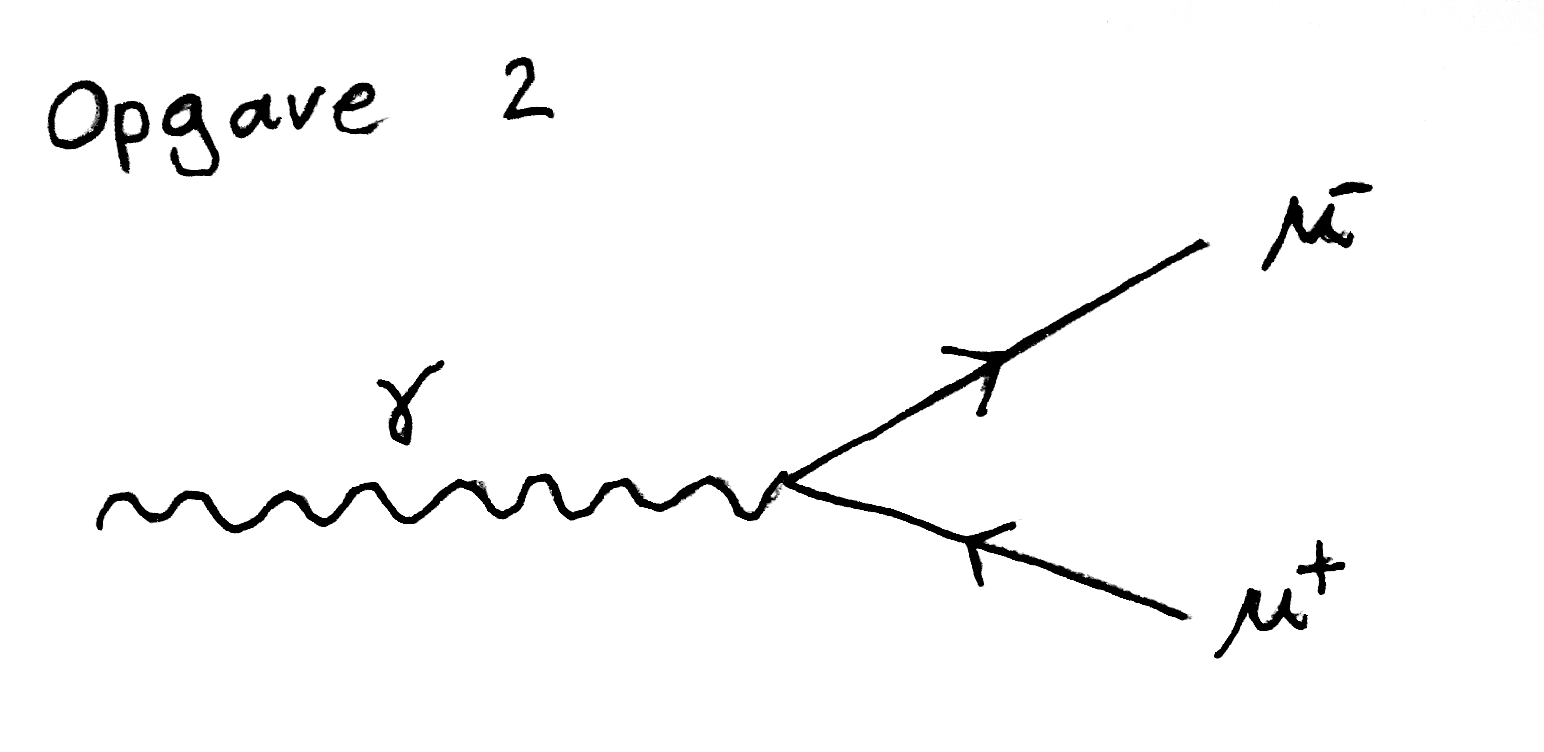
\includegraphics[width=0.4\textwidth]{KernePartikel/opg2.png}
  \caption{Muon pardannelse}
  \label{fig:opg2}
\end{figure}
En muon har hvilemassen $105,7$ \si{MeV/c^2}. Energien for at danne et par er derfor givet ved:
\begin{align*}
E &= 2 m_{\mu} c^2 \\
&= 211,4~\si{MeV} = 3,38~ 10^{-17} \si{J}
\end{align*}
\end{opgave}

\begin{opgave}{Reaktioner med $W^\pm$-partiklen}{2}
\label{opg:W}
\opg
\begin{figure}[h]
  \centering
  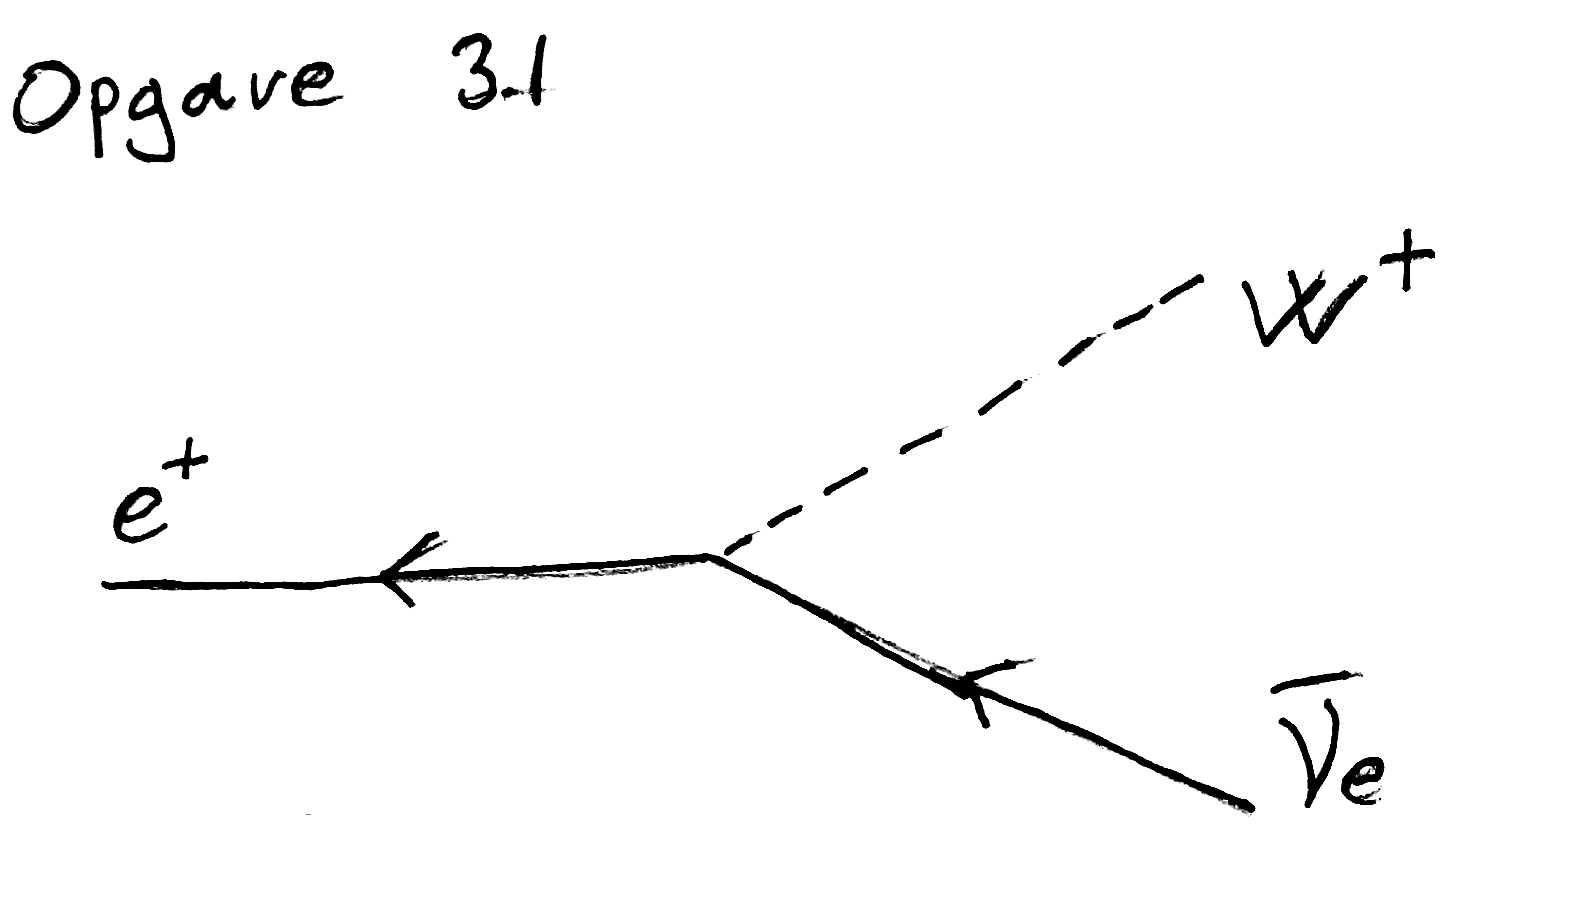
\includegraphics[width=0.4\textwidth]{KernePartikel/opg31.png}
  \caption{Rotation af Feynmandiagram.}
  \label{fig:opg31}
\end{figure}
Se figur \ref{fig:opg31}.
\bigskip
Elektronen bliver til en positron og elektronneutrinoen bliver til en anti-elektronneutrino.
\opg
\begin{figure}[h]
  \centering
  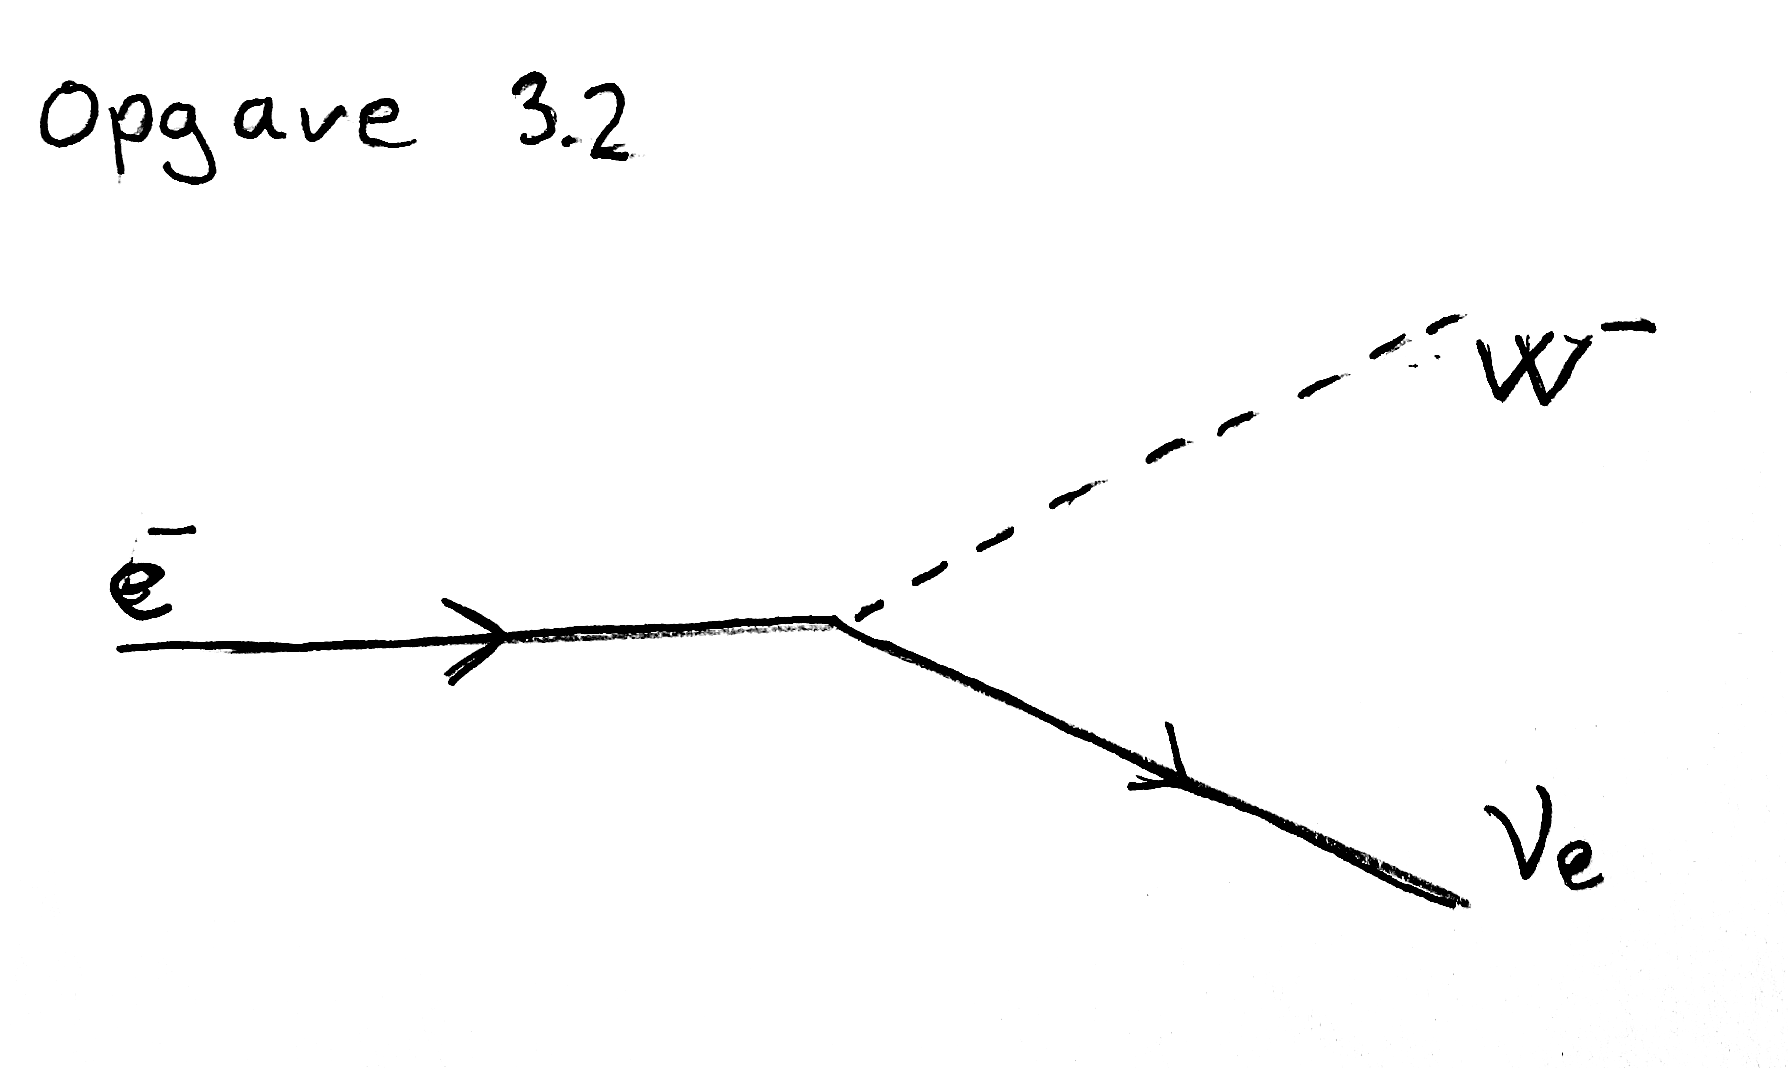
\includegraphics[width=0.4\textwidth]{KernePartikel/opg32.png}
  \caption{Elektron i stedet for positron som indgang.}
  \label{fig:opg32}
\end{figure}
Se figur \ref{fig:opg32}.
\bigskip
Positronen bliver til en electron og anti-elektronneutrinoen bliver til en elektronneutrino.
\opg Feynman-diagrammet for et beta-plus-henfald: $p \rightarrow
n + e^+ + \nu_e$.
\begin{figure}[h]
  \centering
  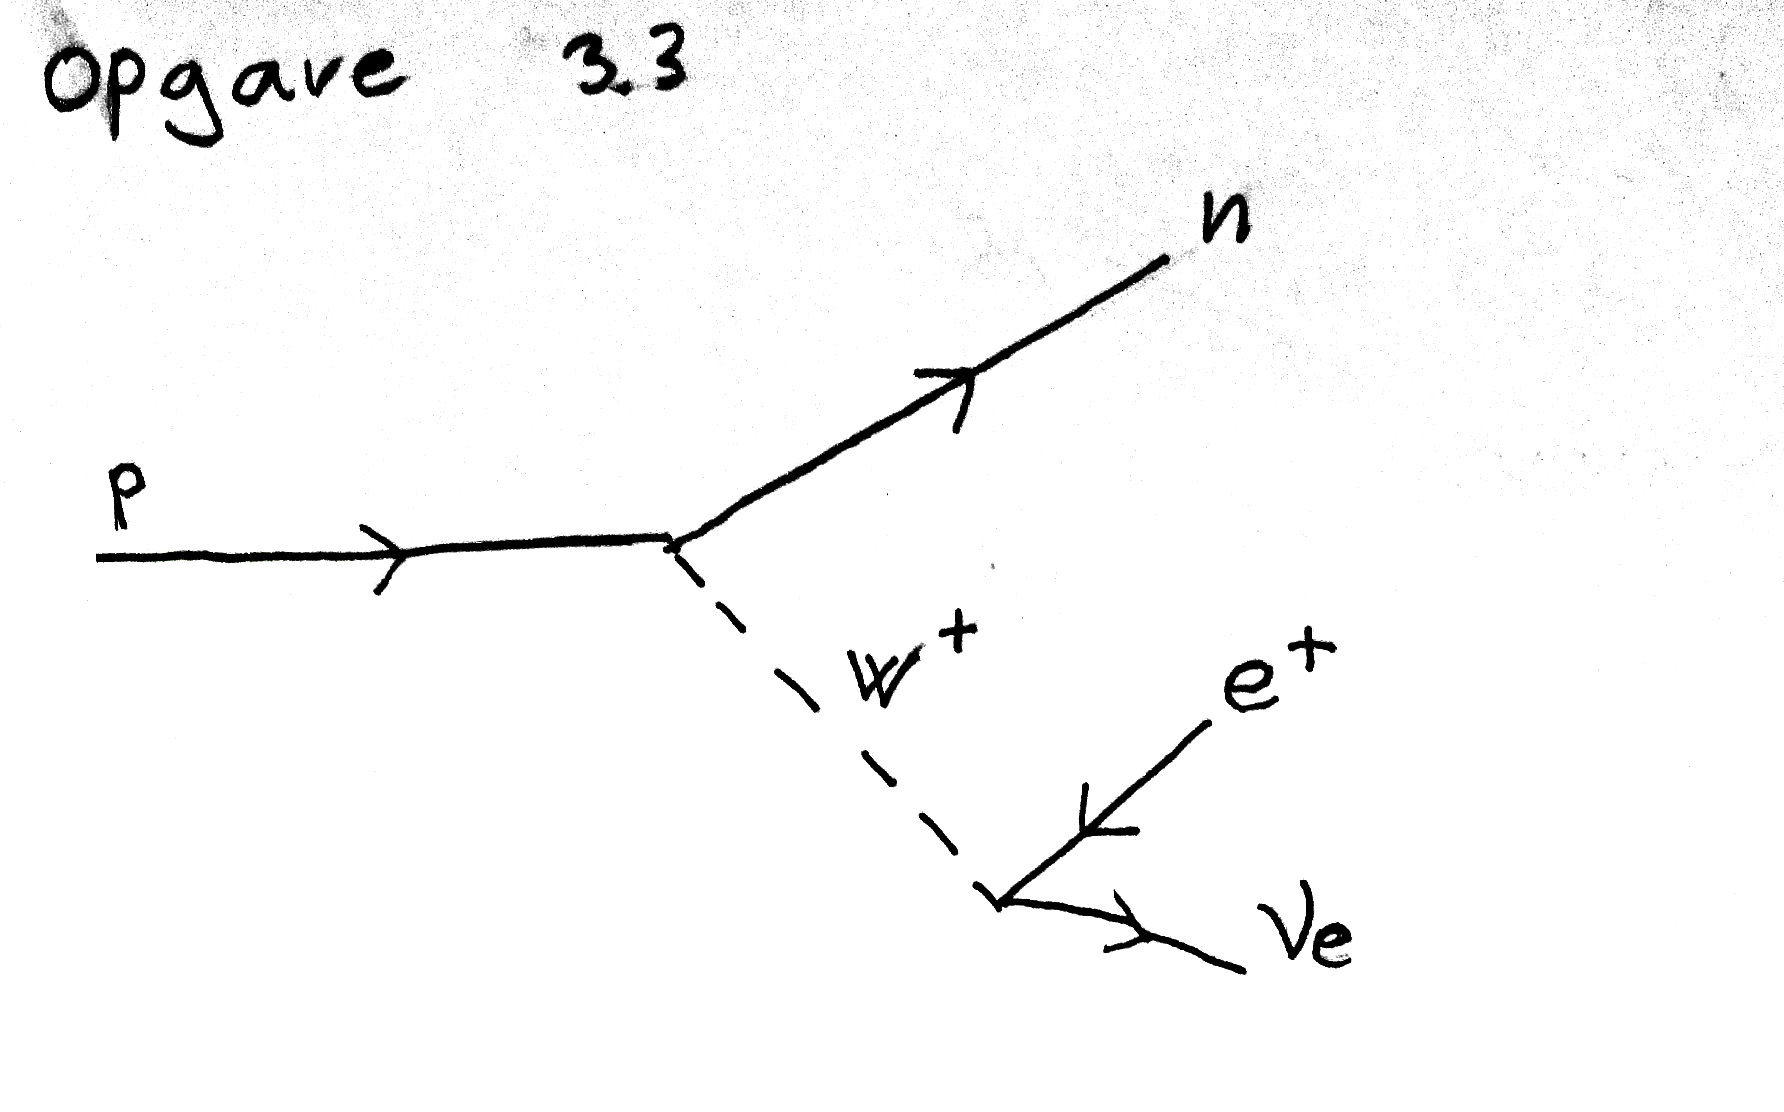
\includegraphics[width=0.4\textwidth]{KernePartikel/opg33.png}
  \caption{Beta plus henfald}
  \label{fig:opg33}
\end{figure}
Se figur \ref{fig:opg33}.
\bigskip
Protonen bliver til en neutron under udsendelse af en $W^+$-partikel, der henfalder til et positron-elektronneutrino-par.
\opg Tegn feynman-diagrammet for en elektron-indfangning: $p + e^-
\rightarrow n + \nu_e$.
\begin{figure}[h]
  \centering
  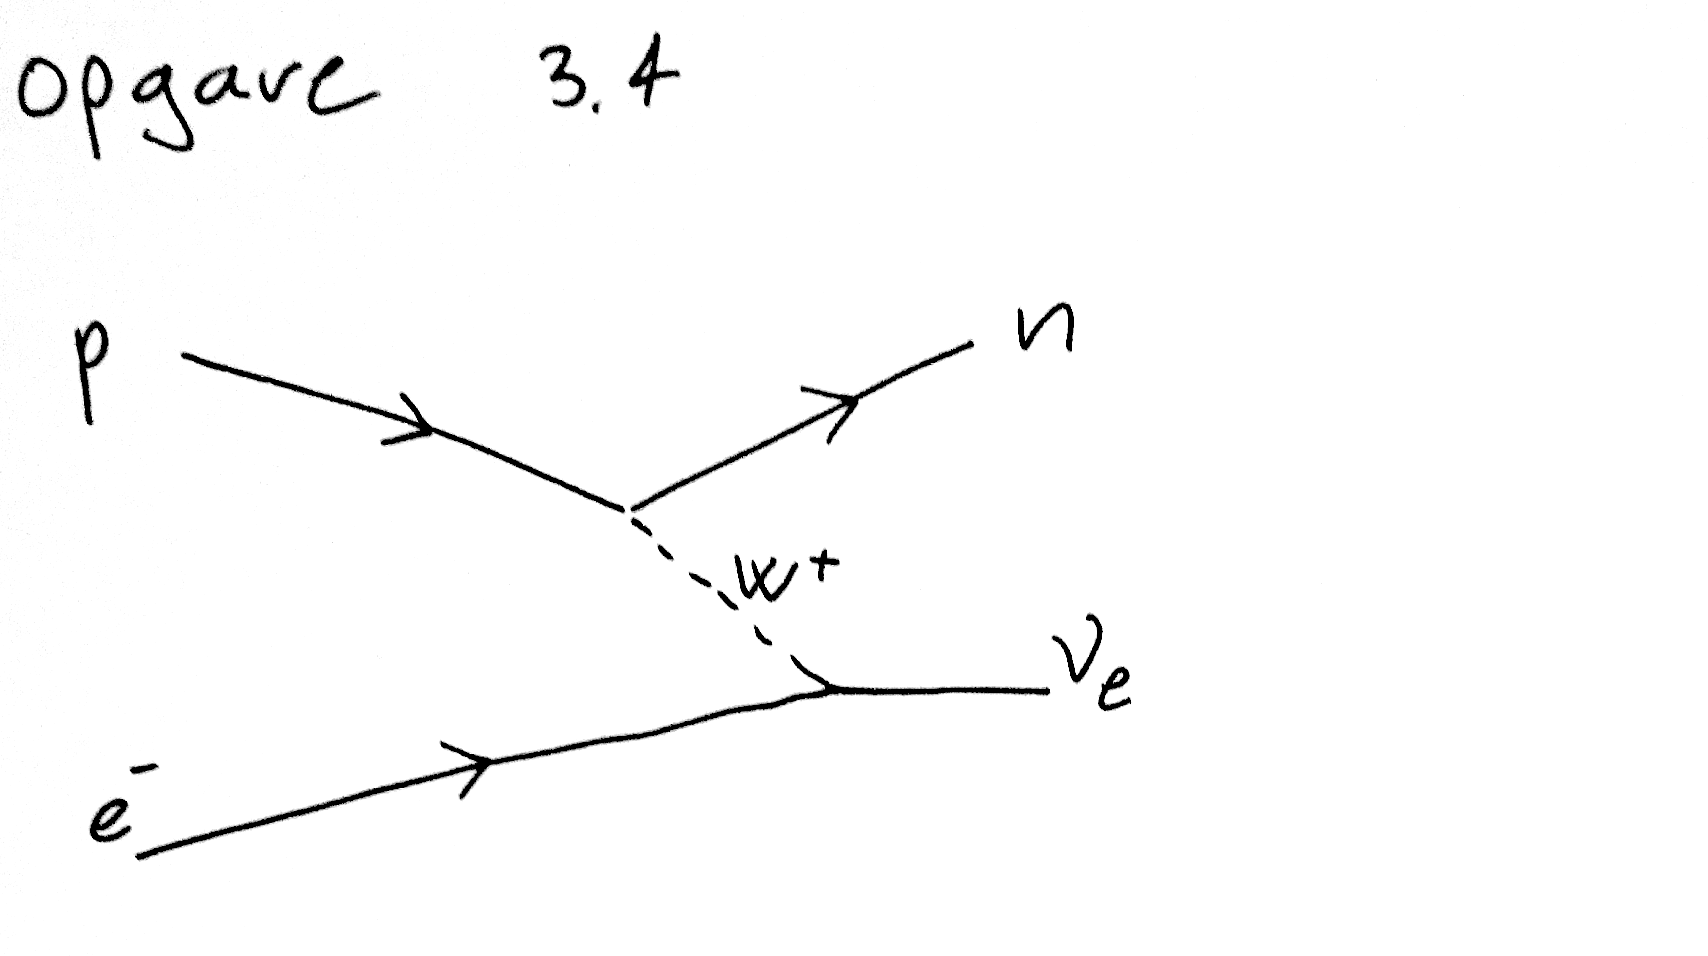
\includegraphics[width=0.4\textwidth]{KernePartikel/opg34.png}
  \caption{Elektron-indfangning}
  \label{fig:opg34}
\end{figure}
Se figur \ref{fig:opg34}.
\bigskip
Processen sker i to trin: udsendelsen af en W-boson fra protonen under omdannelse til en neutron. W-bosonen kan møde elektronen og danne en elektron-neutrino.
\opg Indtegn på figur \ref{fig:Wquarks} pile mellem alle de kvarker, som $W$ kan omdanne. 
\begin{figure}[h]
  \centering
  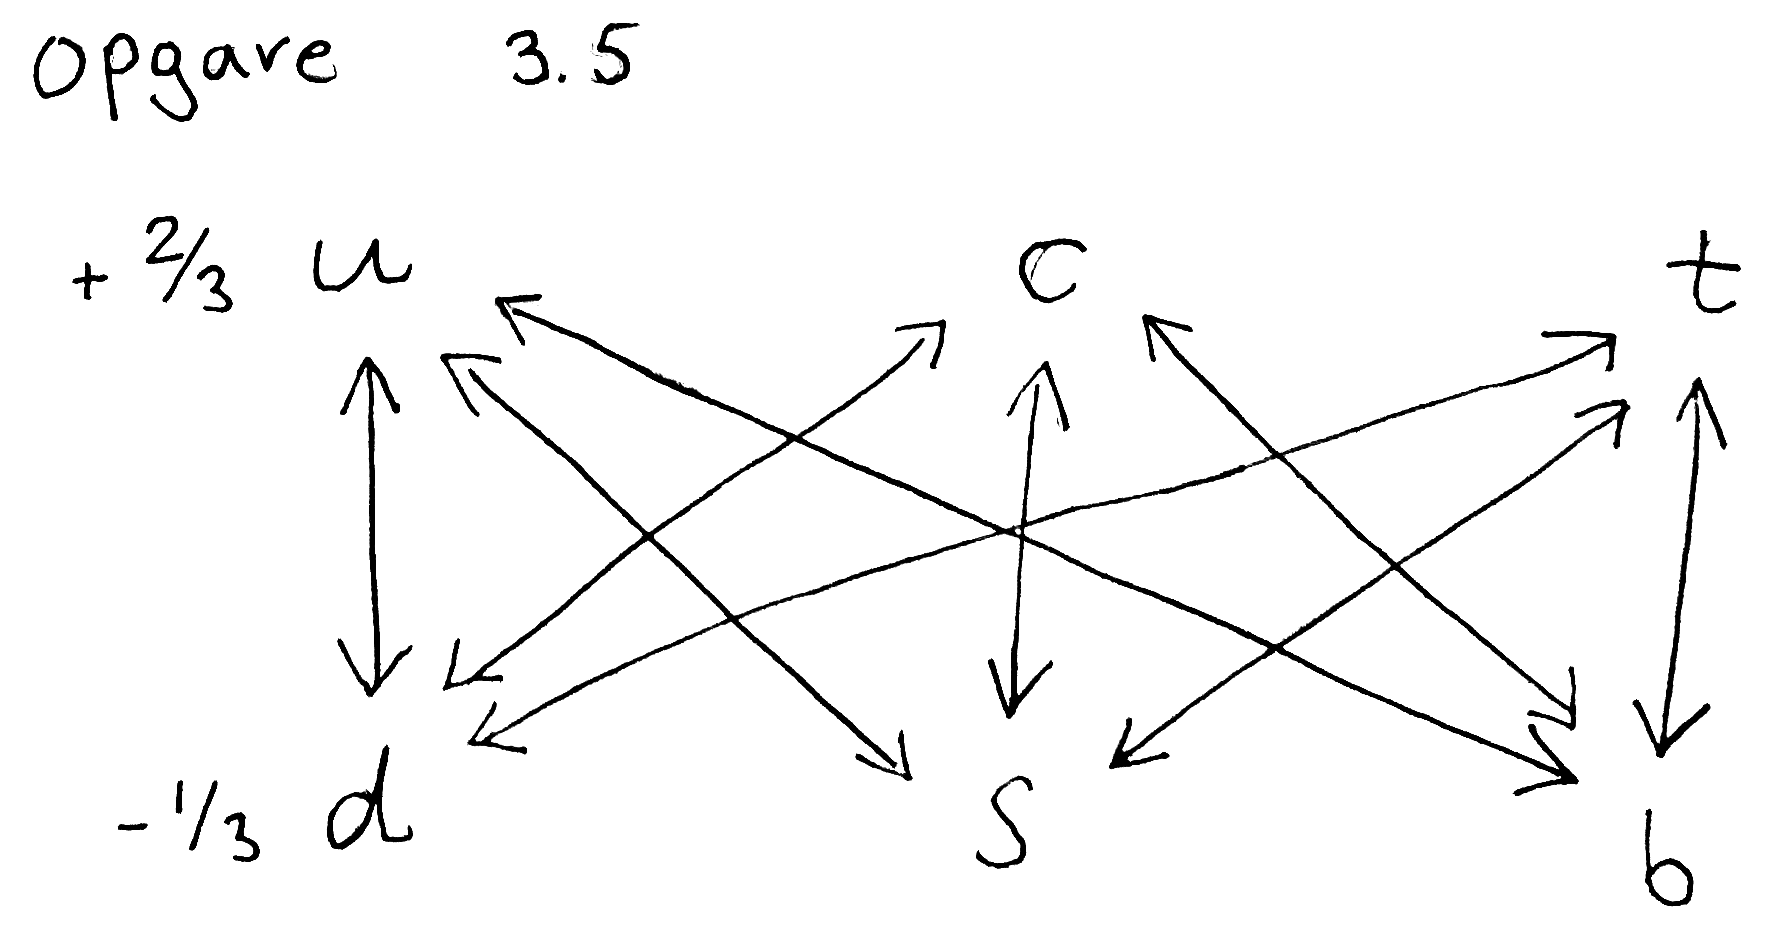
\includegraphics[width=0.4\textwidth]{KernePartikel/opg35.png}
  \caption{Kvarkomdannelser, som $W$ kan lave.}
  \label{fig:opg35}
\end{figure}
Se figur \ref{fig:opg35}.
\opg 
\begin{figure}[h]
  \centering
  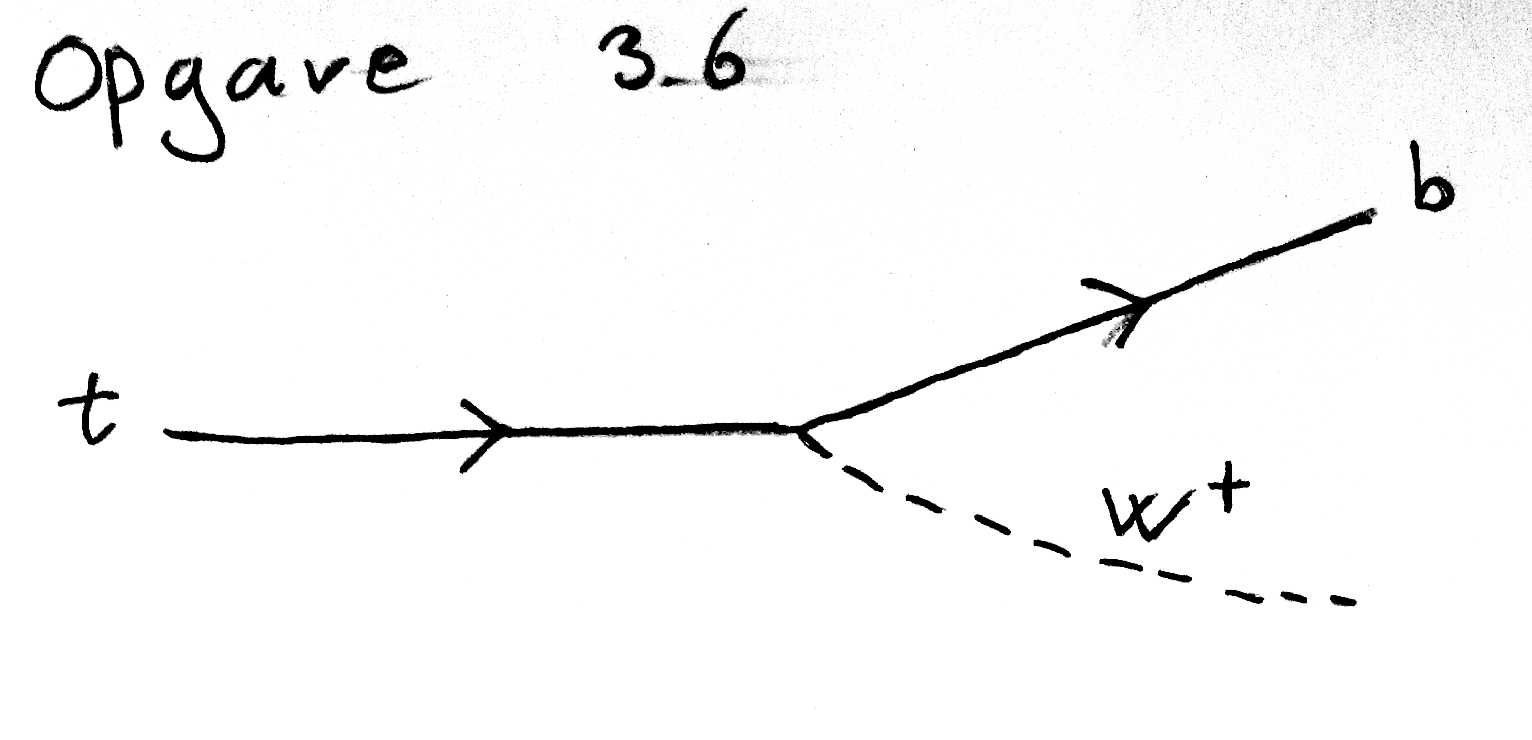
\includegraphics[width=0.4\textwidth]{KernePartikel/opg36.png}
  \caption{t-kvark omdannes til b-kvark.}
  \label{fig:opg36}
\end{figure}
Se figur \ref{fig:opg36}.
\bigskip
Ladningen af $W$ er +1.
\opg 
\begin{figure}[h]
  \centering
  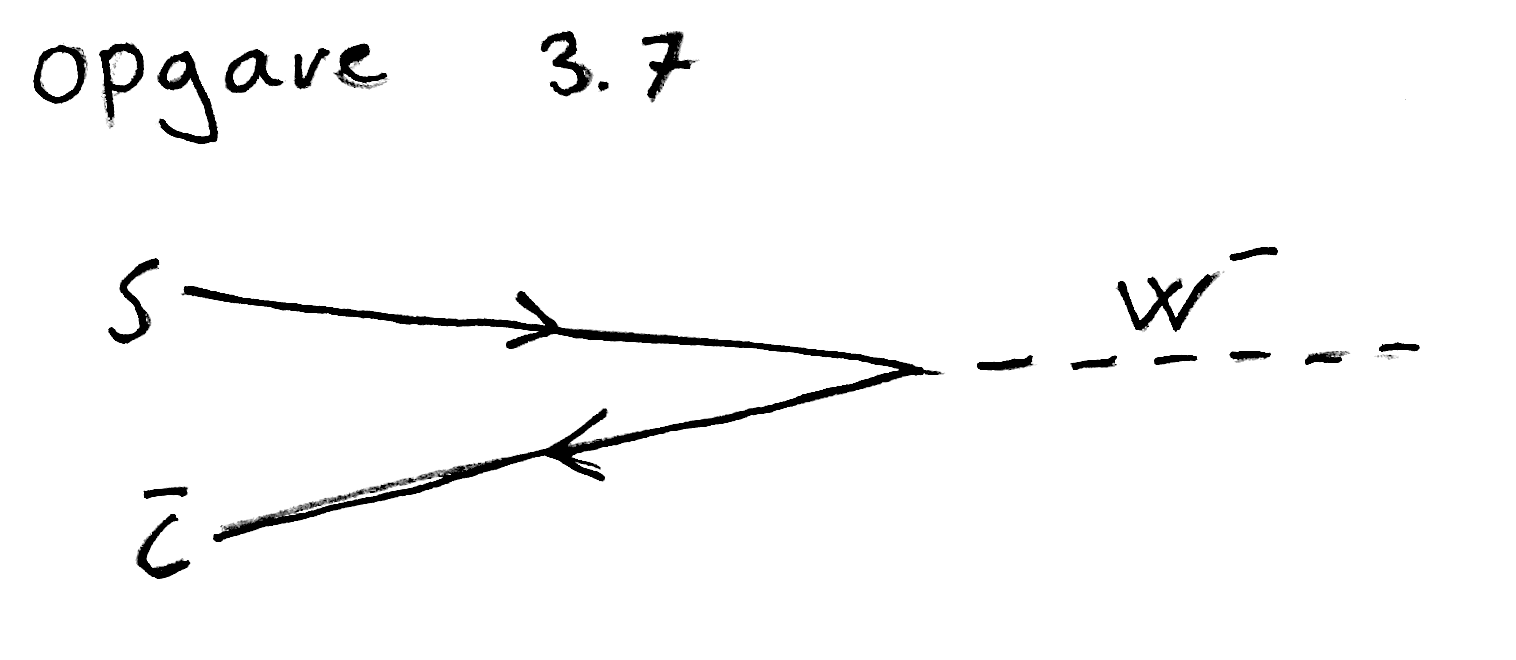
\includegraphics[width=0.4\textwidth]{KernePartikel/opg37.png}
  \caption{s-kvark og anti-c kvark annihilerer.}
  \label{fig:opg37}
\end{figure}
Se figur \ref{fig:opg37}.
\bigskip
Ladningen af $W$ er -1.
\opg 
\begin{figure}[h]
  \centering
  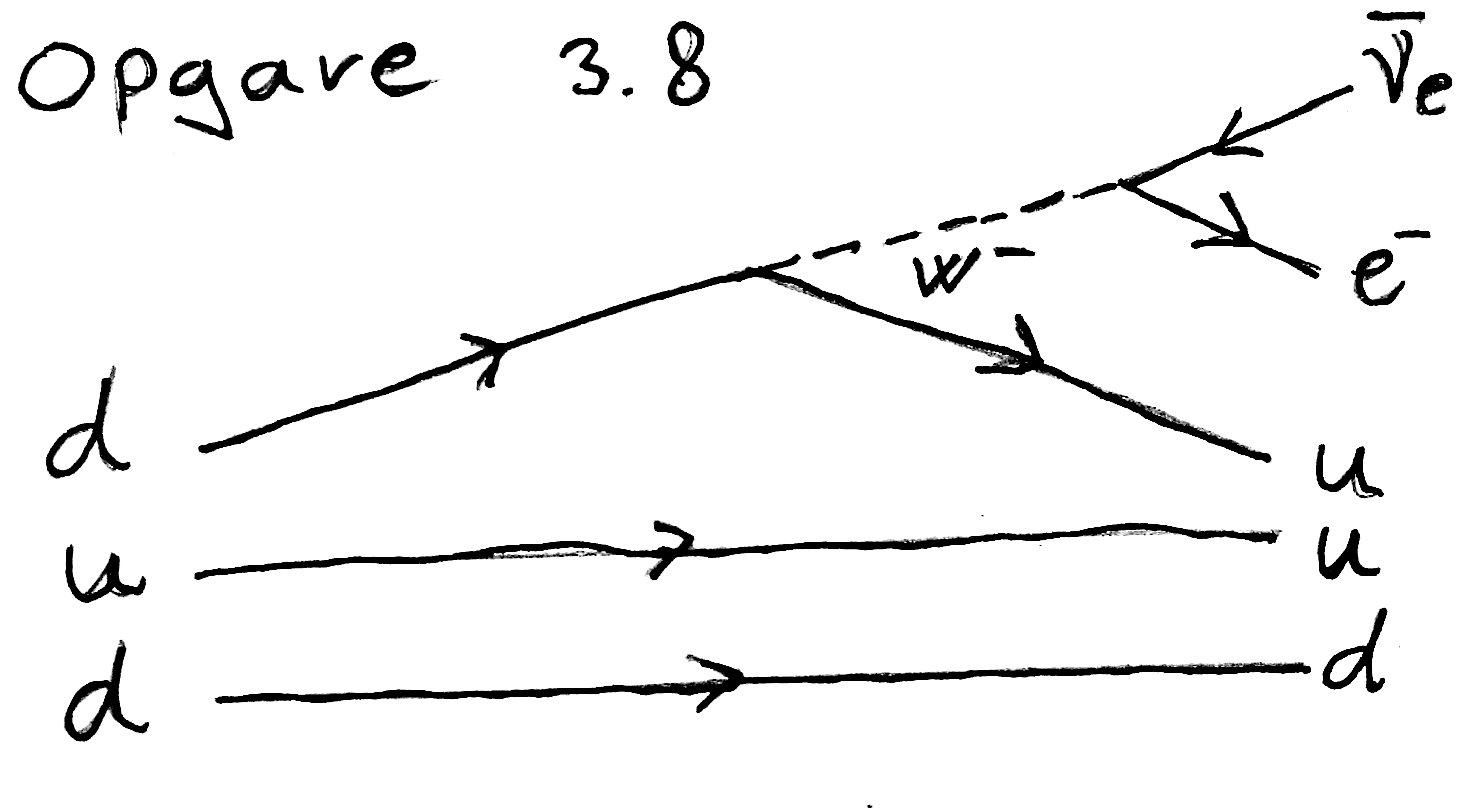
\includegraphics[width=0.4\textwidth]{KernePartikel/opg38.png}
  \caption{Beta minus henfald.}
  \label{fig:opg38}
\end{figure}
Se figur \ref{fig:opg38}.
\end{opgave}


\begin{opgave}{Feynman-diagrammer: en sand kunstart}{3}
\label{opg:feynman1}
\opg Ladningen af $W$ er -1.
\opg Den ene kvark udsender en gluon og passerer derefter uændret. Gluonen henfalder til et kvark/anti-kvark-par. Den anden kvark i $D^-$-mesonen ændres under udsendelse af en $W^-1$. Denne $W^-$ henfalder og skaber to nye kvarker.
\opg 
\begin{figure}[h]
  \centering
  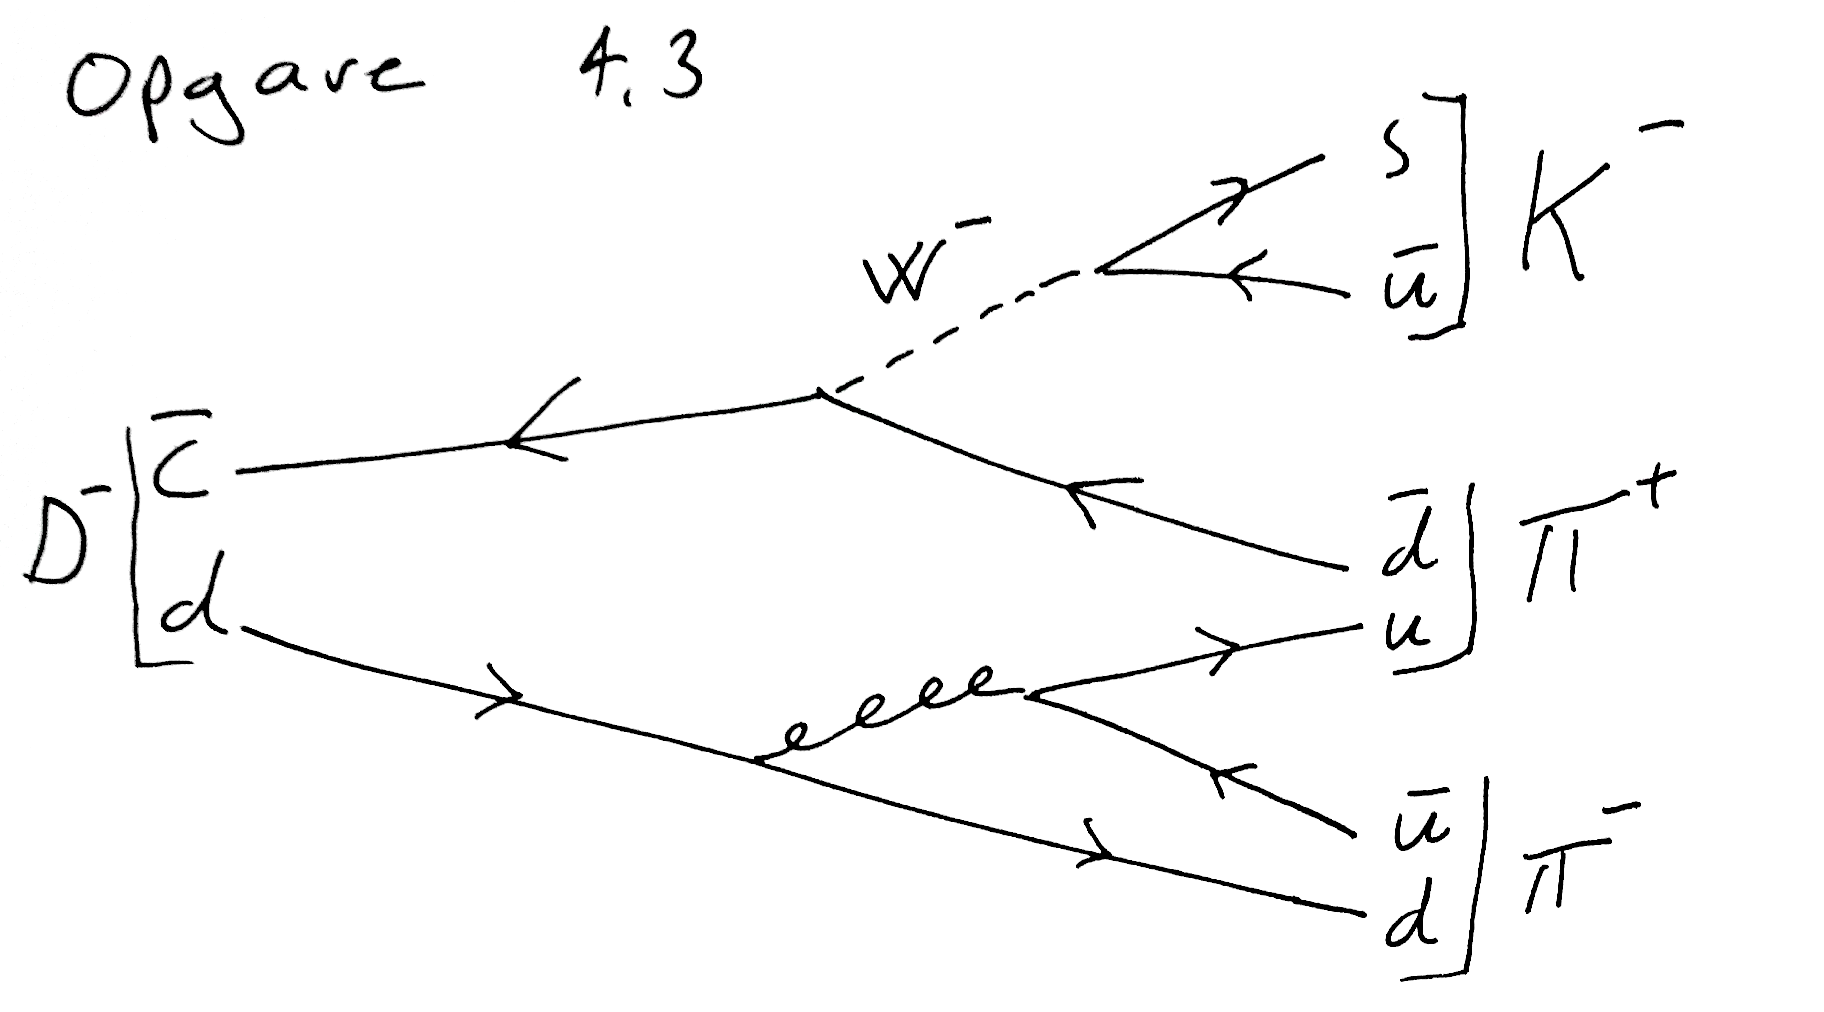
\includegraphics[width=0.4\textwidth]{KernePartikel/opg43.png}
  \caption{Feynmandiagram for henfald af $D^-$-mesonen.}
  \label{fig:opg43}
\end{figure}
Se figur \ref{fig:opg43}.
\bigskip
\end{opgave}

\begin{opgave}{Relativistiske partikler}{2}
\opg 
\begin{align*}
E & = m_\text{rel} c^2 \\
E & = \frac{m}{\sqrt{1-v^2/c^2}} c^2 \\
v/c & = \sqrt{1-\frac{m^2 c^4}{E^2}} \\
&= 0,99999961
\end{align*}
\opg Den relativistiske masse er allerede givet af opgaven gennem Einstein\'s formel $E=mc^2$:
\begin{align*}
m_\text{rel} & = 580~\si{MeV/c^2} = 1,03~ 10^{-27} ~\si{kg}
\end{align*}
\end{opgave}

\begin{opgave}{Flere feynman-diagrammer}{2}
\opg $B^- (b\bar{u}) \longrightarrow D^0(c\bar{u}) + \rho^-(d\bar{u})$
\begin{figure}[h]
  \centering
  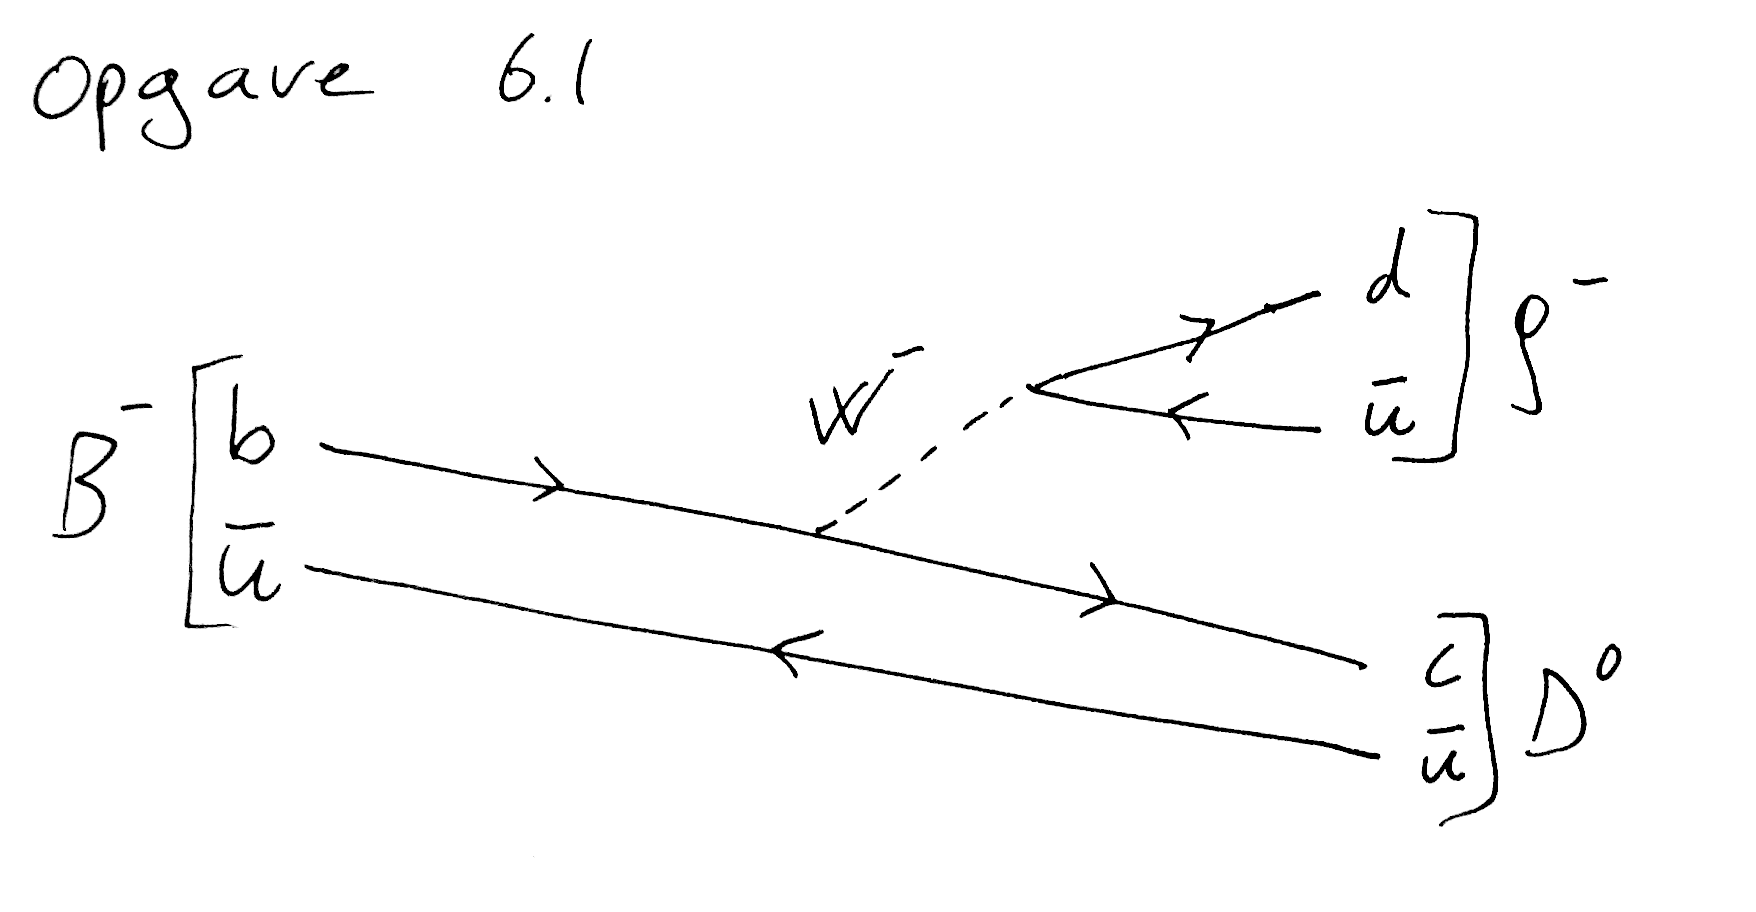
\includegraphics[width=0.4\textwidth]{KernePartikel/opg61.png}
  \caption{Feynmandiagram for henfald af $B^-$.}
  \label{fig:opg61}
\end{figure}
Se figur \ref{fig:opg61}.
\opg $\Sigma^-(dds) \longrightarrow \Lambda^0 (uds) + e^- + \bar{\nu}_e$
\begin{figure}[h]
  \centering
  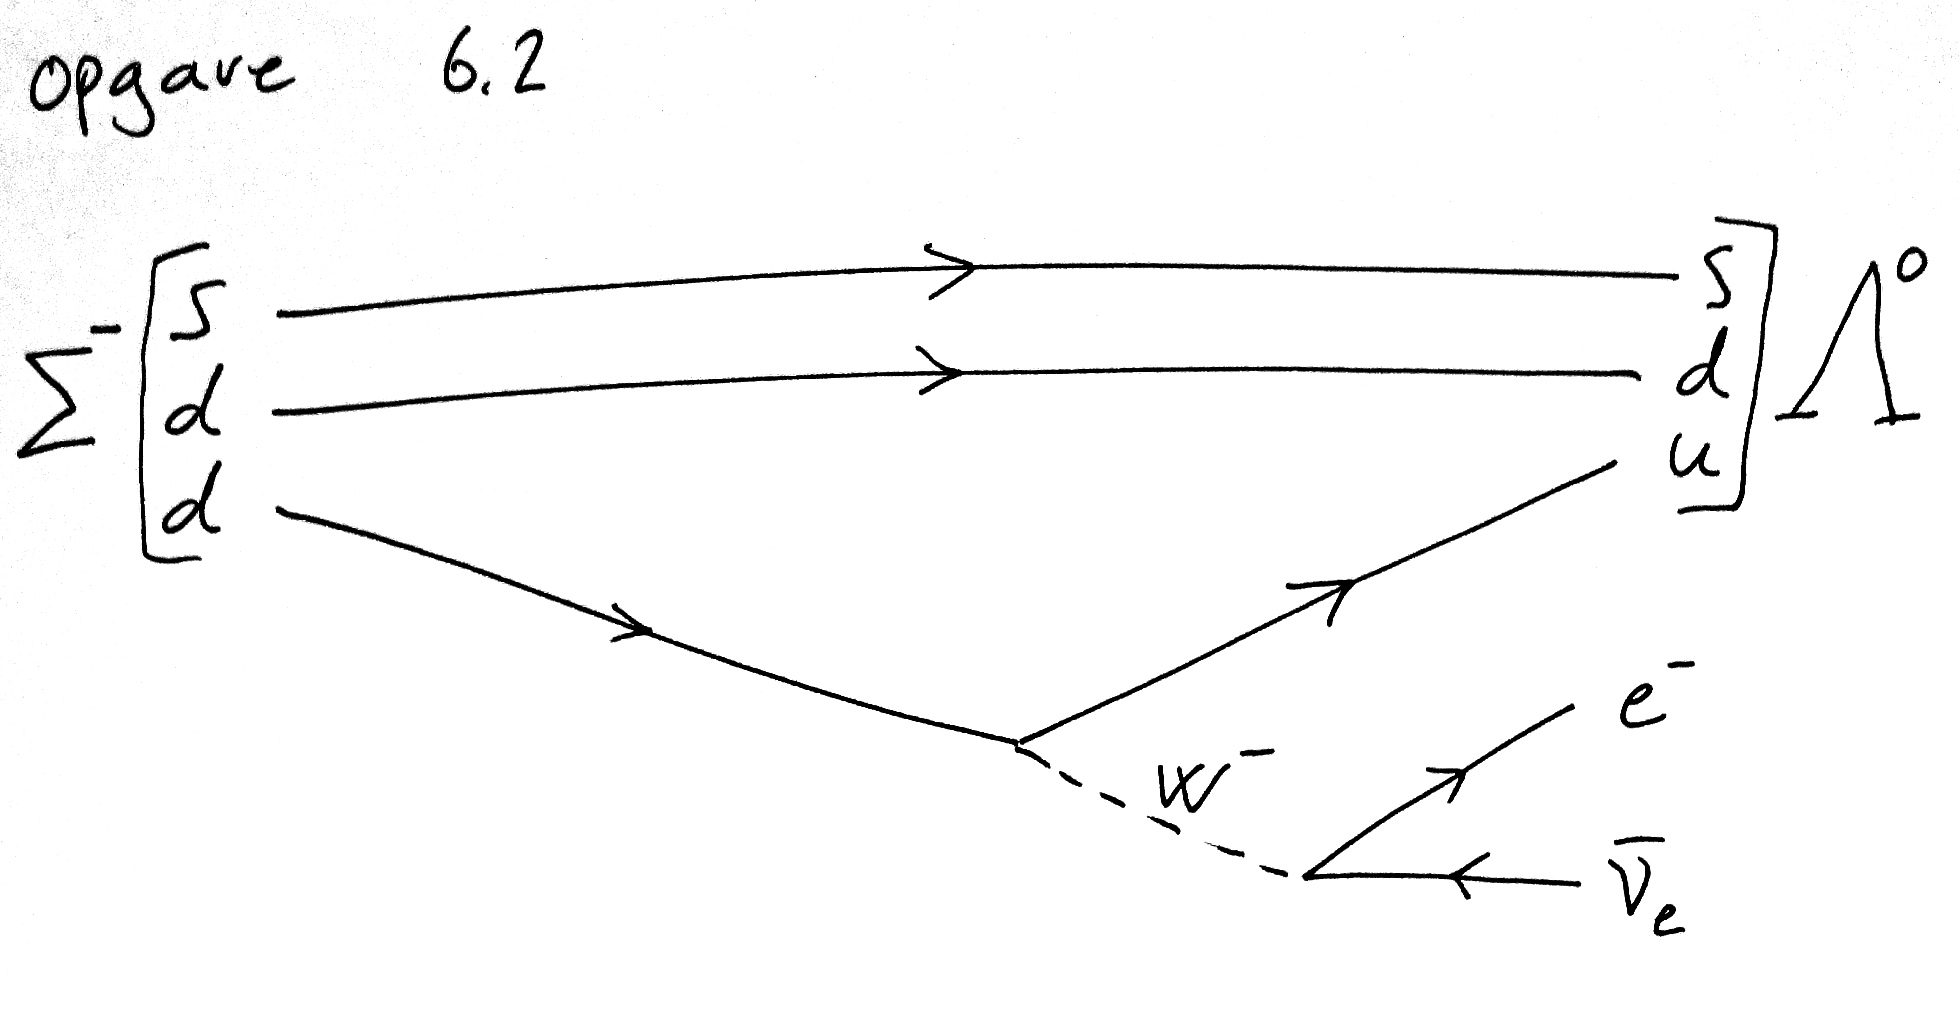
\includegraphics[width=0.4\textwidth]{KernePartikel/opg62.png}
  \caption{Feynmandiagram for henfald af $\Sigma^-$.}
  \label{fig:opg62}
\end{figure}
Se figur \ref{fig:opg62}.
\opg $\Delta^0 (udd) \longrightarrow p + \pi^- (d\bar{u})$
\begin{figure}[h]
  \centering
  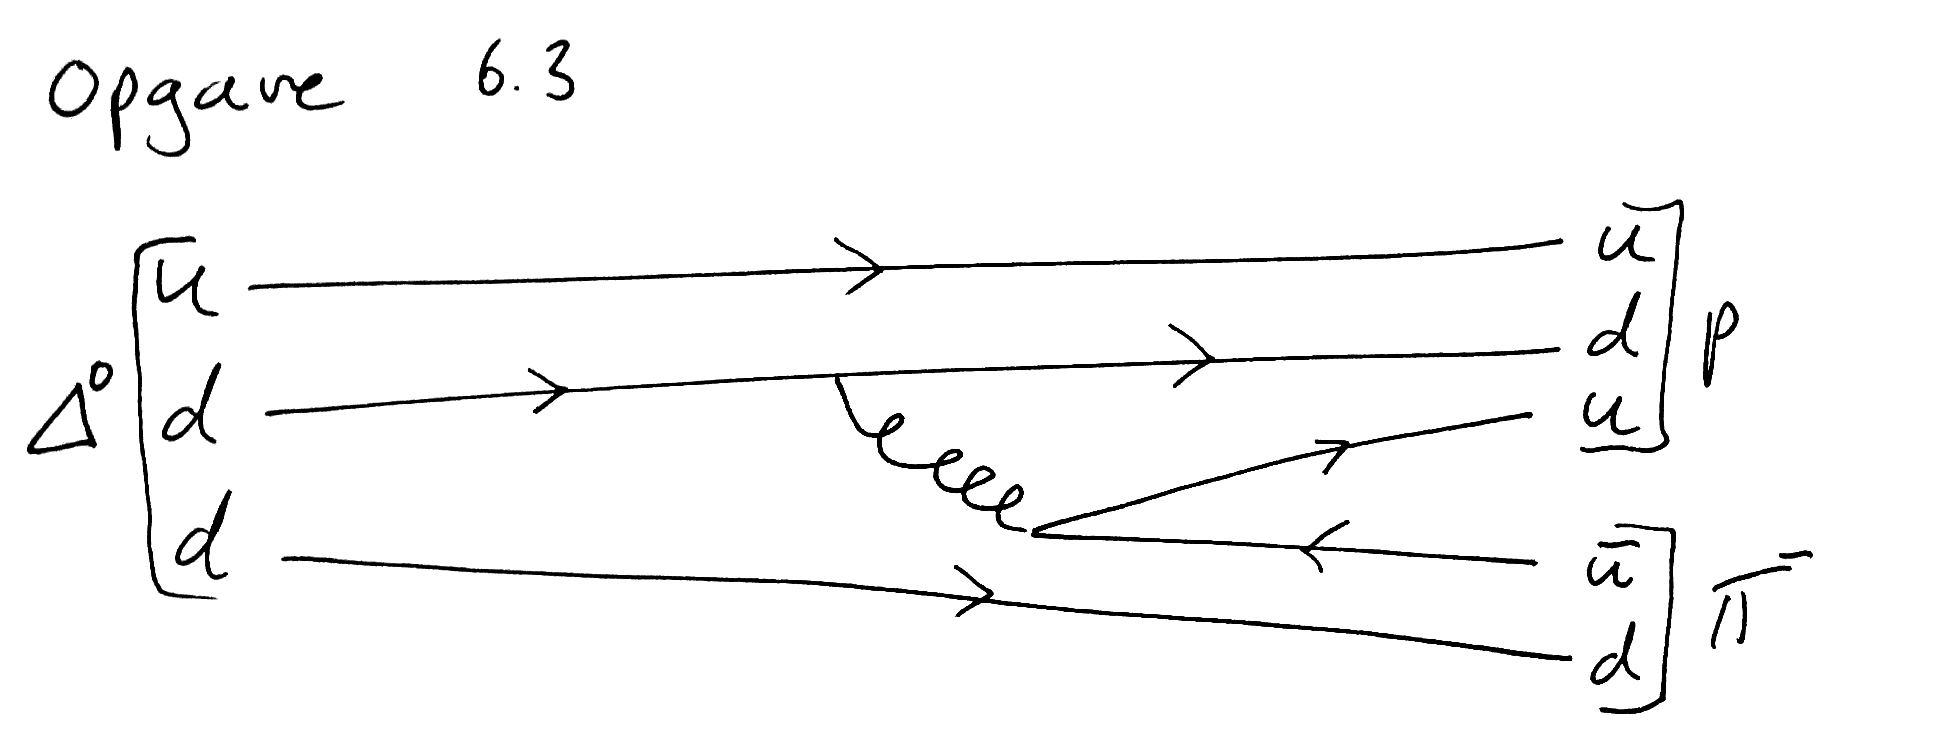
\includegraphics[width=0.4\textwidth]{KernePartikel/opg63.png}
  \caption{Feynmandiagram for henfald af $\Delta^0$.}
  \label{fig:opg63}
\end{figure}
Se figur \ref{fig:opg63}.
\opg $D_s^+ (c\bar{s}) \longrightarrow \phi (s\bar{s}) + \rho^+ (u\bar{d})$
\begin{figure}[h]
  \centering
  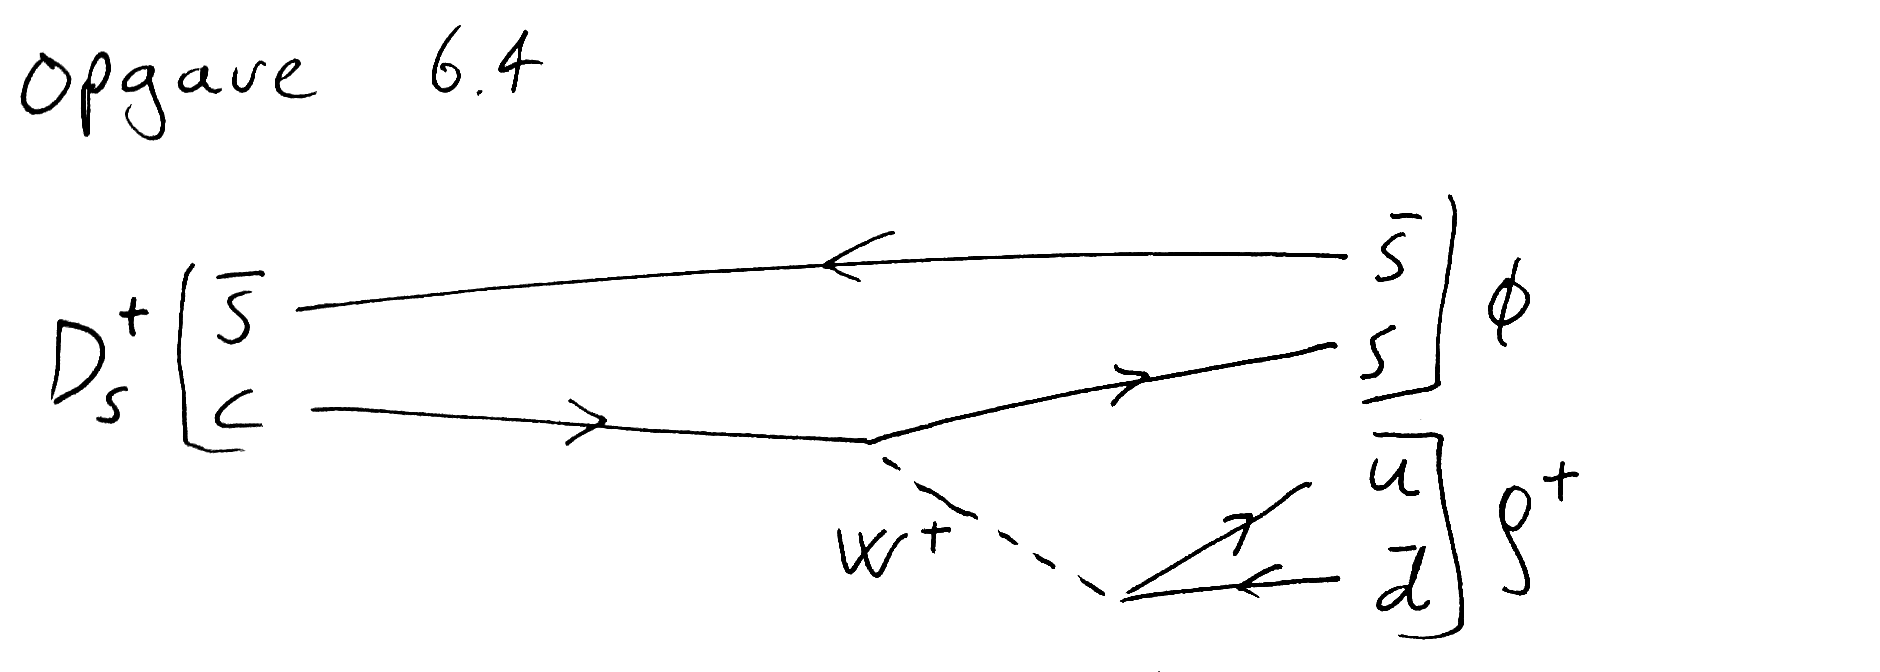
\includegraphics[width=0.4\textwidth]{KernePartikel/opg64.png}
  \caption{Feynmandiagram for henfald af $D^{+}_{s}$.}
  \label{fig:opg64}
\end{figure}
Se figur \ref{fig:opg64}.
\opg $\Omega^-(sss) \longrightarrow \Xi^-(dss) + \pi^0(u\bar{u})$
\begin{figure}[h]
  \centering
  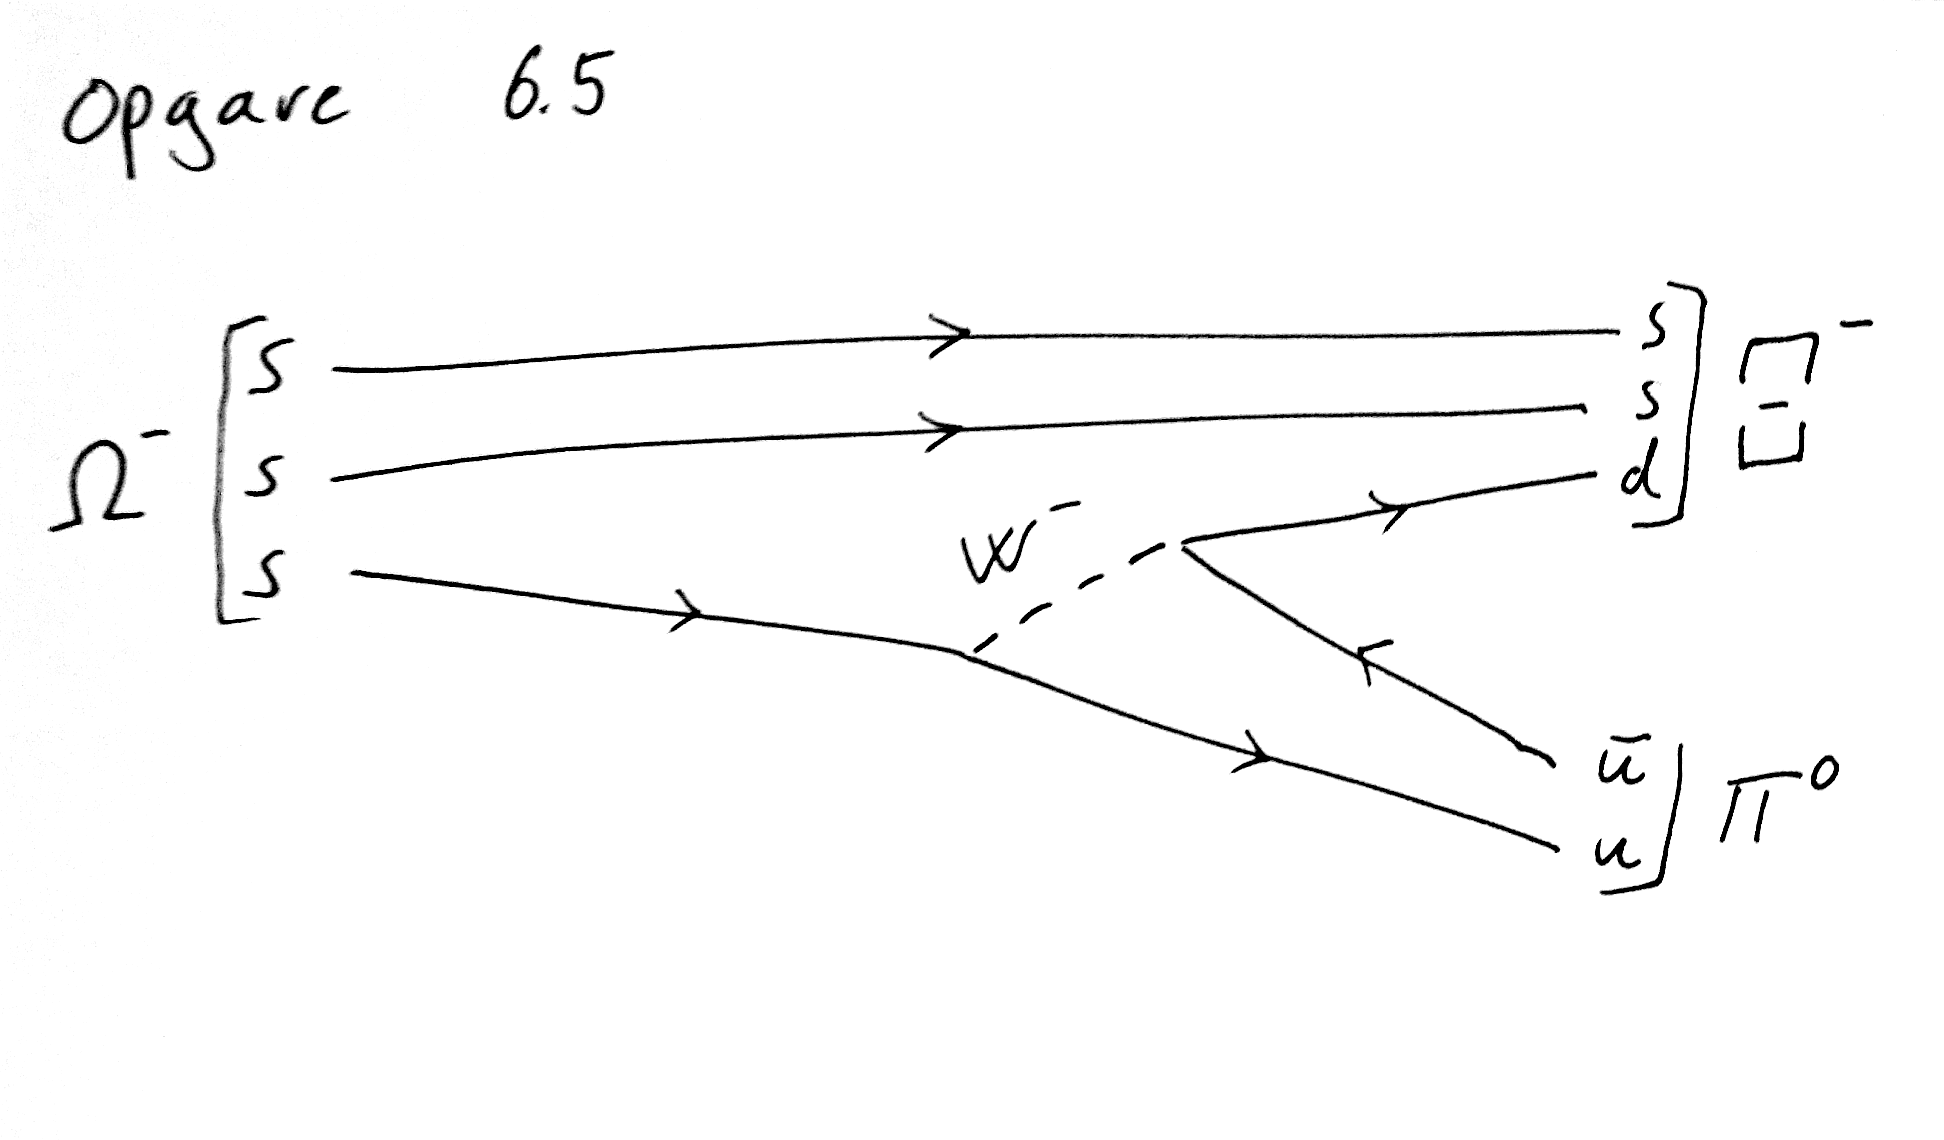
\includegraphics[width=0.4\textwidth]{KernePartikel/opg65.png}
  \caption{Feynmandiagram for henfald af $\Omega^-$.}
  \label{fig:opg65}
\end{figure}
Se figur \ref{fig:opg65}.
\end{opgave}